\documentclass{beamer}
\usetheme{metropolis}           % Use metropolis theme
\usepackage{appendixnumberbeamer}
\usepackage{epigraph}
\usepackage{color}
\usepackage{amsopn}
\usepackage{tabto}
\usepackage{pbox}           % table line break
\usepackage{algorithm}      % algorithm
\usepackage[noend]{algpseudocode} % algorithm
\usepackage{bm}             % bold in math
\usepackage{mathtools}      % dcases*

%%% Bibliography
\usepackage[backend=bibtex, style=authoryear]{biblatex}
\AtBeginBibliography{\tiny}
\bibliography{../bibliography.bib}

\setcounter{tocdepth}{1}      % hide subsections in Table of Contents
\renewcommand{\thealgorithm}{} % disable numbering of algorithms

\setbeamercolor{background canvas}{bg=white}
\setbeamercolor{title}{fg=gray!10}
\setbeamercolor{subtitle}{fg=gray!15}
\setbeamercolor{author}{fg=gray!40}
\setbeamercolor{date}{fg=gray!60}
\setbeamercolor{institute}{fg=gray!20}

\newcommand{\todo}{\alert{TODO}}
\newcommand{\itemBullet}{\scriptsize$\blacksquare$}
\setbeamertemplate{itemize item}{\itemBullet}
\setbeamertemplate{itemize subitem}{\itemBullet}
\setbeamertemplate{itemize subsubitem}{\itemBullet}
\newcommand{\E}{\mathop{\mathbb{E}}}
\DeclareMathOperator*{\argmax}{arg\,max}
\newcommand{\epiParSpace}{\vskip 1.5ex}
\newcommand{\p}{\mathbf{p}}
\newcommand{\colorcite}{\color{gray!35}}

\title{Dynamic Routing Between Capsules}
\subtitle{by S. Sabour, N. Frosst and G. Hinton (NIPS 2017)}
\author{presented by Karel Ha}
\date{27\textsuperscript{th} March 2018}                         % no dates
\institute{Pattern Recognition and Computer Vision Reading Group}

\begin{document}
  {
    \usebackgroundtemplate{
      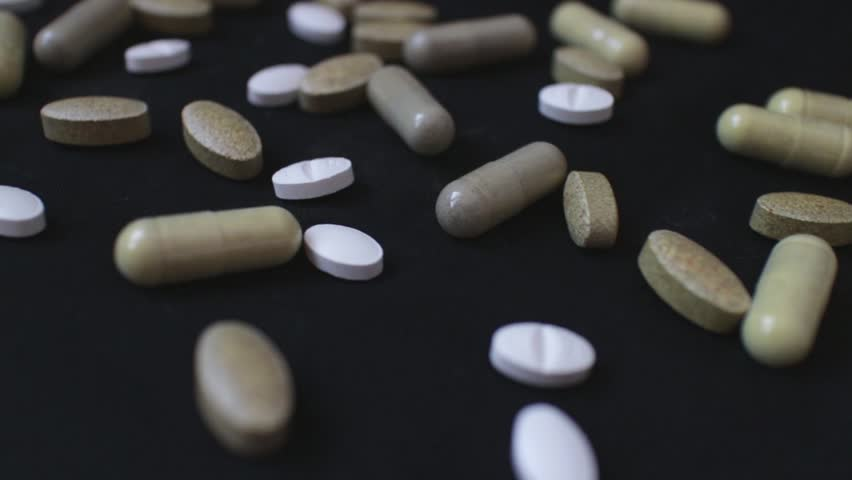
\includegraphics[height=\paperheight]{../img/capsule-pills.jpg}
    }
    \maketitle
  }

  \begin{frame}{Outline}
    \tableofcontents
  \end{frame}

%%%%%%%%%%%%%%%%%%%%%%%%%%%%%%%%%%%%%%%%%%%%%%%%%%%%%%%%%%%%%%%%%%%%%%%%%%%%%%%%

  \section{Motivation}
  {
    \setbeamertemplate{frame footer}{\colorcite\url{http://condo.ca/wp-content/uploads/2017/03/Vector-director-Institute-artificial-intelligence-Toronto-MaRS-Discovery-District-Hinton-Google-Apple-Siri-Alexa-Condo.ca_.jpg}}

    \usebackgroundtemplate{
      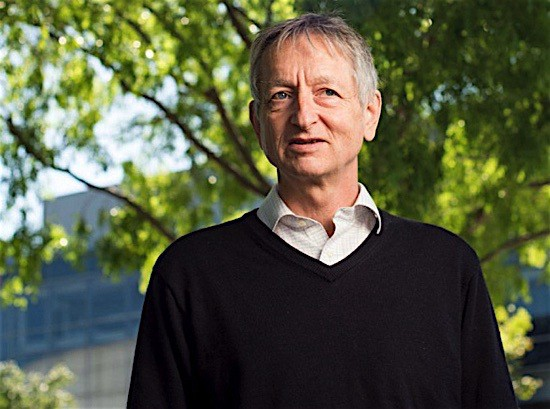
\includegraphics[height=\paperheight]{../img/hinton.jpeg}
    }
    \begin{frame}[standout]
      \color{gray!15}

      \vskip .4\textheight
      \epigraph{
        \tiny
        The pooling operation used in~convolutional neural networks is a~big mistake and the fact that it works so well is a~disaster.
      }{G. Hinton}
      \pause

      \epigraph{
        \tiny
        [...] it makes much more sense to represent a~pose as a~small matrix that converts a~vector of~positional coordinates relative to the viewer into positional coordinates relative to the shape itself.
      }{G. Hinton}
    \end{frame}
  }

  {
    \setbeamertemplate{frame footer}{\colorcite\url{https://medium.com/ai³-theory-practice-business/understanding-hintons-capsule-networks-part-i-intuition-b4b559d1159b}}

    \begin{frame}{Part-Whole Geometric Relationships \\
        \tiny ``What is wrong with convolutional neural nets?''}
      \pause
      \begin{center}
        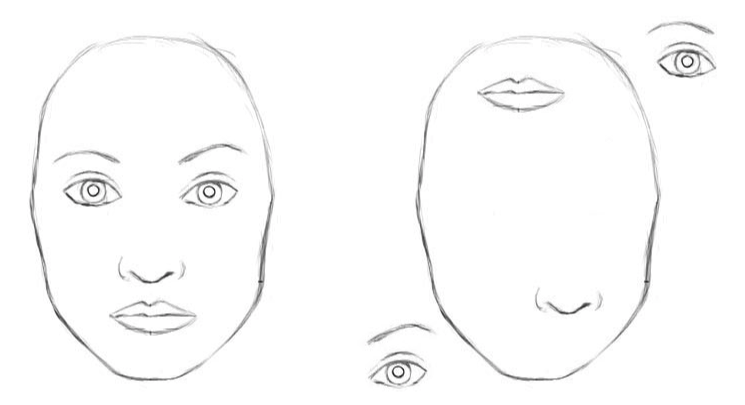
\includegraphics[width=.9\textwidth]{../img/ambiguous-faces.png}
      \end{center}

      \vskip -2em
      \tiny
      To a~CNN (with MaxPool)...
      \pause
      \begin{itemize}[<+- | alert@+>]
        \item ...both pictures are similar, since they both contain similar elements.
        \item ...a mere presence of objects can be a very \textbf{strong indicator} to consider a face in the image.
        \item ...orientational and relative spatial relationships are not very important.
      \end{itemize}
    \end{frame}
  }

  {
    \setbeamertemplate{frame footer}{\colorcite\url{http://math.hws.edu/graphicsbook/c2/scene-graph.png}}

    \begin{frame}{Part-Whole Geometric Relationships \\
        \tiny Scene Graphs from Computer Graphics}
      \pause
      \tiny
      ...takes into account relative positions of objects.

      \begin{center}
        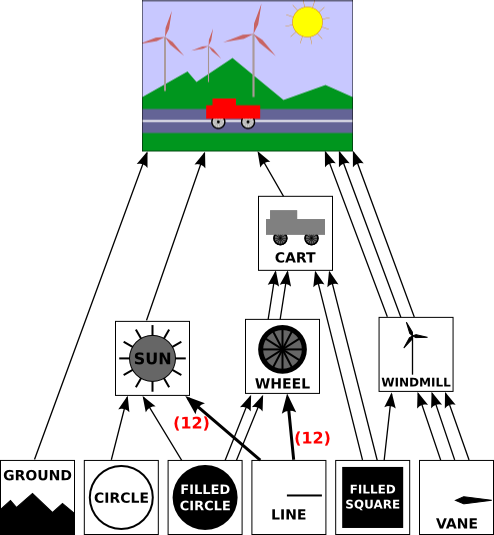
\includegraphics[height=.6\textheight]{../img/scene-graph.png}
      \end{center}
      \pause
      \vskip -1em
      The internal representation in computer memory:
      \pause
      \vskip -1em
      \begin{enumerate}[a)]
        \item arrays of~geometrical objects
          \pause
        \item matrices representing their \textbf{relative positions} and \textbf{orientations}
      \end{enumerate}
    \end{frame}
  }

  {
    \setbeamertemplate{frame footer}{\colorcite\url{https://d1jnx9ba8s6j9r.cloudfront.net/blog/wp-content/uploads/2017/12/CNN-Capsule-Networks-Edureka-442x300.png}}

    \begin{frame}{Part-Whole Geometric Relationships \\
        \tiny Inverse (Computer) Graphics}
      \begin{center}
        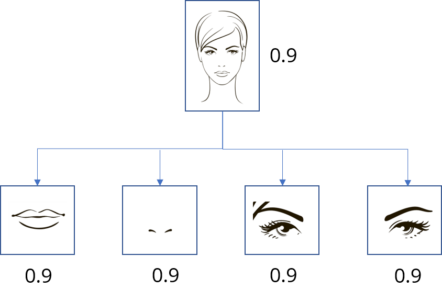
\includegraphics[height=.5\textheight]{../img/reverse-rendering.png}
      \end{center}
      \pause

      \tiny
      Inverse graphics:
      \pause
      \begin{itemize}[<+- | alert@+>]
        \item from visual information received by eyes
        \item deconstruct a~hierarchical representation of the world around us
        \item and try to match it with already learned patterns and relationships stored in the brain
        \item relationships between 3D objects using a~\textbf{``pose''} (= translation plus rotation)
      \end{itemize}
    \end{frame}
  }

  {
    \setbeamertemplate{frame footer}{\colorcite\url{https://medium.com/ai³-theory-practice-business/understanding-hintons-capsule-networks-part-i-intuition-b4b559d1159b}}

    \begin{frame}{Pose Equivariance and the Viewing Angle}
      \pause
      We have probably never seen these exact pictures, but we can still immediately recognize the object in it...
      \begin{center}
        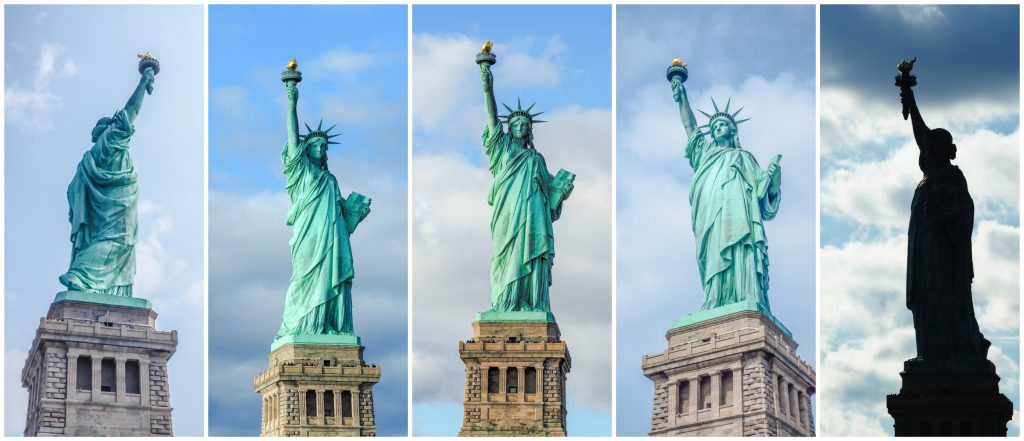
\includegraphics[height=.5\textheight]{../img/statue-of-liberty.jpeg}
      \end{center}

      \pause
      \tiny
      \vskip -1em
      \begin{itemize}[<+- | alert@+>]
        \item internal representation in the brain: independent of the viewing angle
        \item quite hard for a~CNN: no built-in understanding of~3D space
        \item much easier for a~CapsNet: these relationships are explicitly modeled
      \end{itemize}
    \end{frame}
  }

  {
    \setbeamertemplate{frame footer}{\colorcite\url{https://www.oreilly.com/ideas/introducing-capsule-networks}}

    \begin{frame}{Routing by an Agreement: High-Dimensional Coincidence}
      \pause
      \begin{center}
        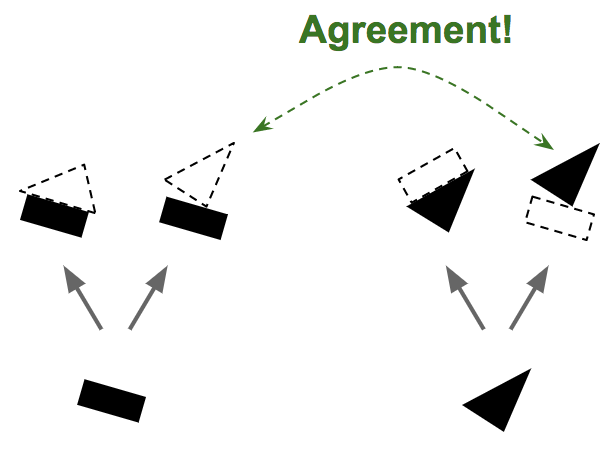
\includegraphics[height=.5\textheight]{../img/routing-agreement.png}
        \pause

        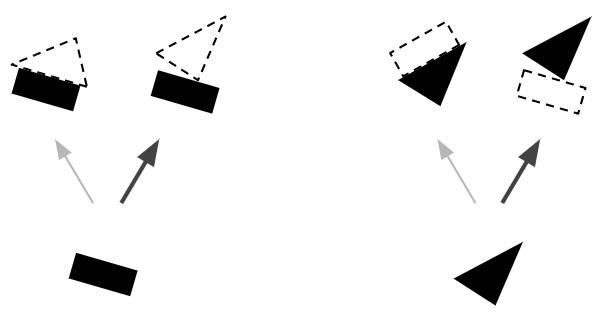
\includegraphics[height=.35\textheight]{../img/routing-weights.png}
      \end{center}
    \end{frame}

    \begin{frame}{Routing by an Agreement: Illustrative Overview}
      \pause
      \begin{center}
        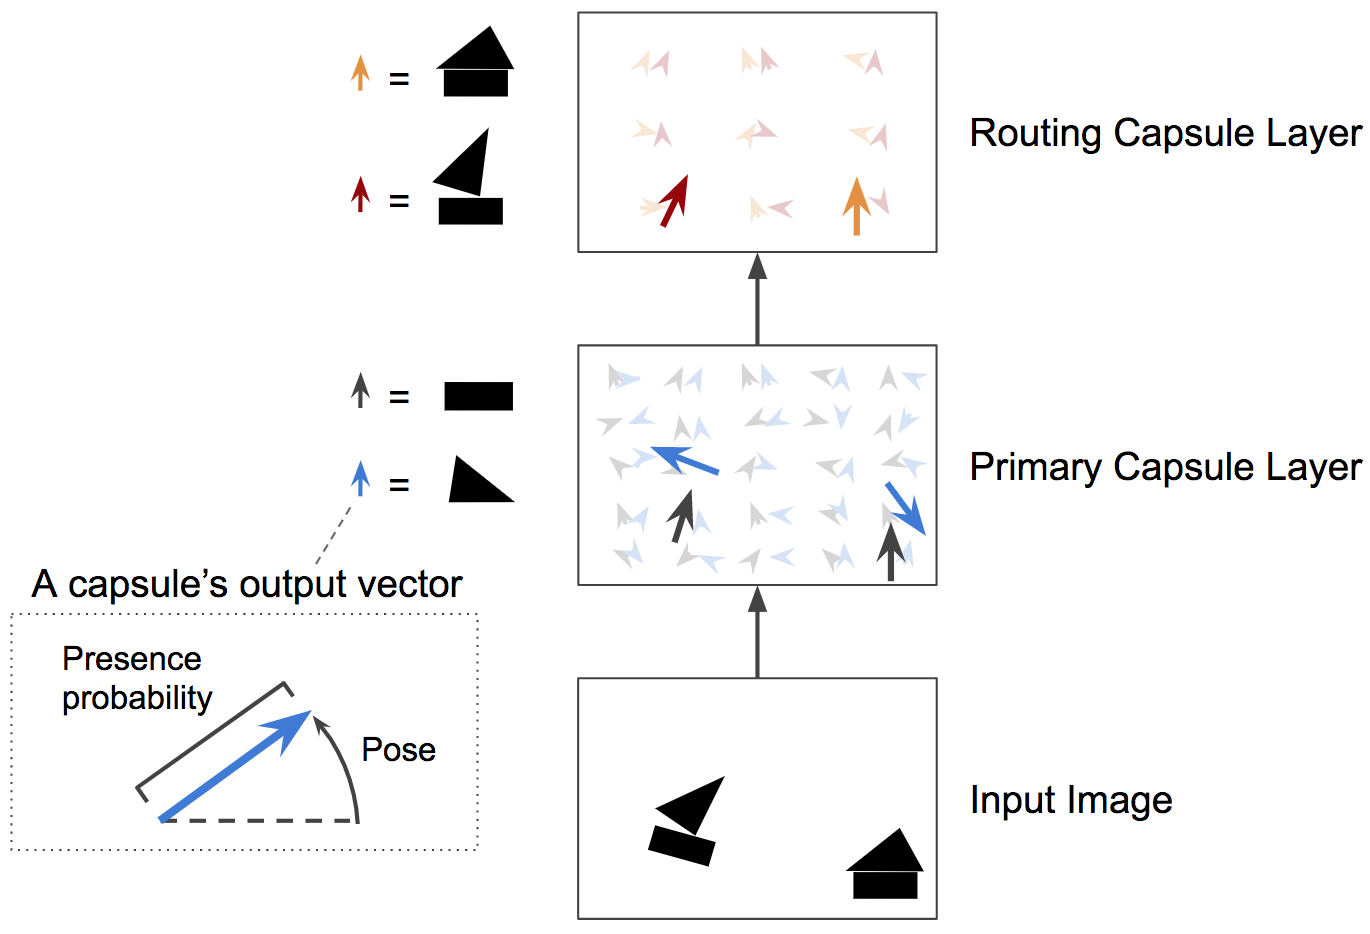
\includegraphics[height=.85\textheight]{../img/routing-by-layers.png}
      \end{center}
    \end{frame}

    \begin{frame}{Routing by an Agreement: Recognizing Ambiguity in Images}
      \begin{center}
        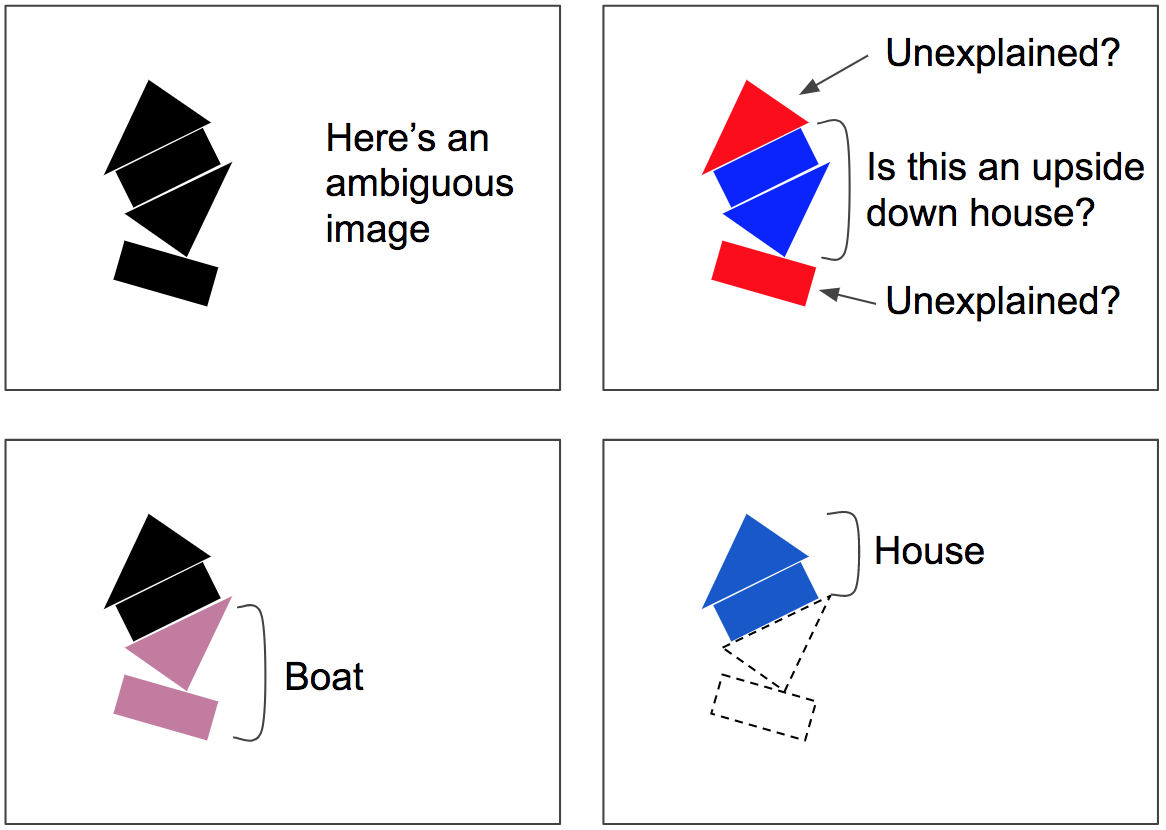
\includegraphics[height=.85\textheight]{../img/ambiguous-shapes.png}
      \end{center}
    \end{frame}
  }

  {
    \setbeamertemplate{frame footer}{\colorcite[\cite{Sabour2017dynamic}]}

    \begin{frame}{Routing: Lower Levels Voting for Higher-Level Feature}
      \begin{center}
        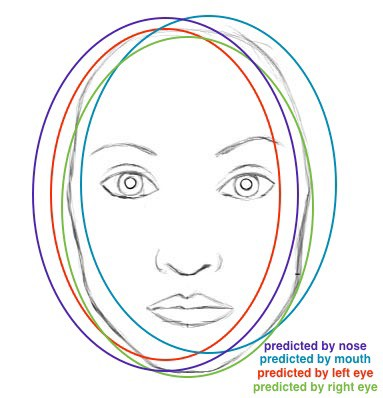
\includegraphics[height=.8\textheight]{../img/hi-dim-coincidence-face.png}
      \end{center}
    \end{frame}
  }

  \begin{frame}[standout]
    How to do it? \\
    (mathematically)
  \end{frame}

%%%%%%%%%%%%%%%%%%%%%%%%%%%%%%%%%%%%%%%%%%%%%%%%%%%%%%%%%%%%%%%%%%%%%%%%%%%%%%%%

  \section{Capsule}

  %\subsection{CapsNets vs ConvNets}
  %{
  %  \setbeamertemplate{frame footer}{\colorcite[\cite{Sabour2017dynamic}]}

  %  \begin{frame}{Where ConvNets Ends... And CapsNets Begins...}
  %    \begin{center}
  %      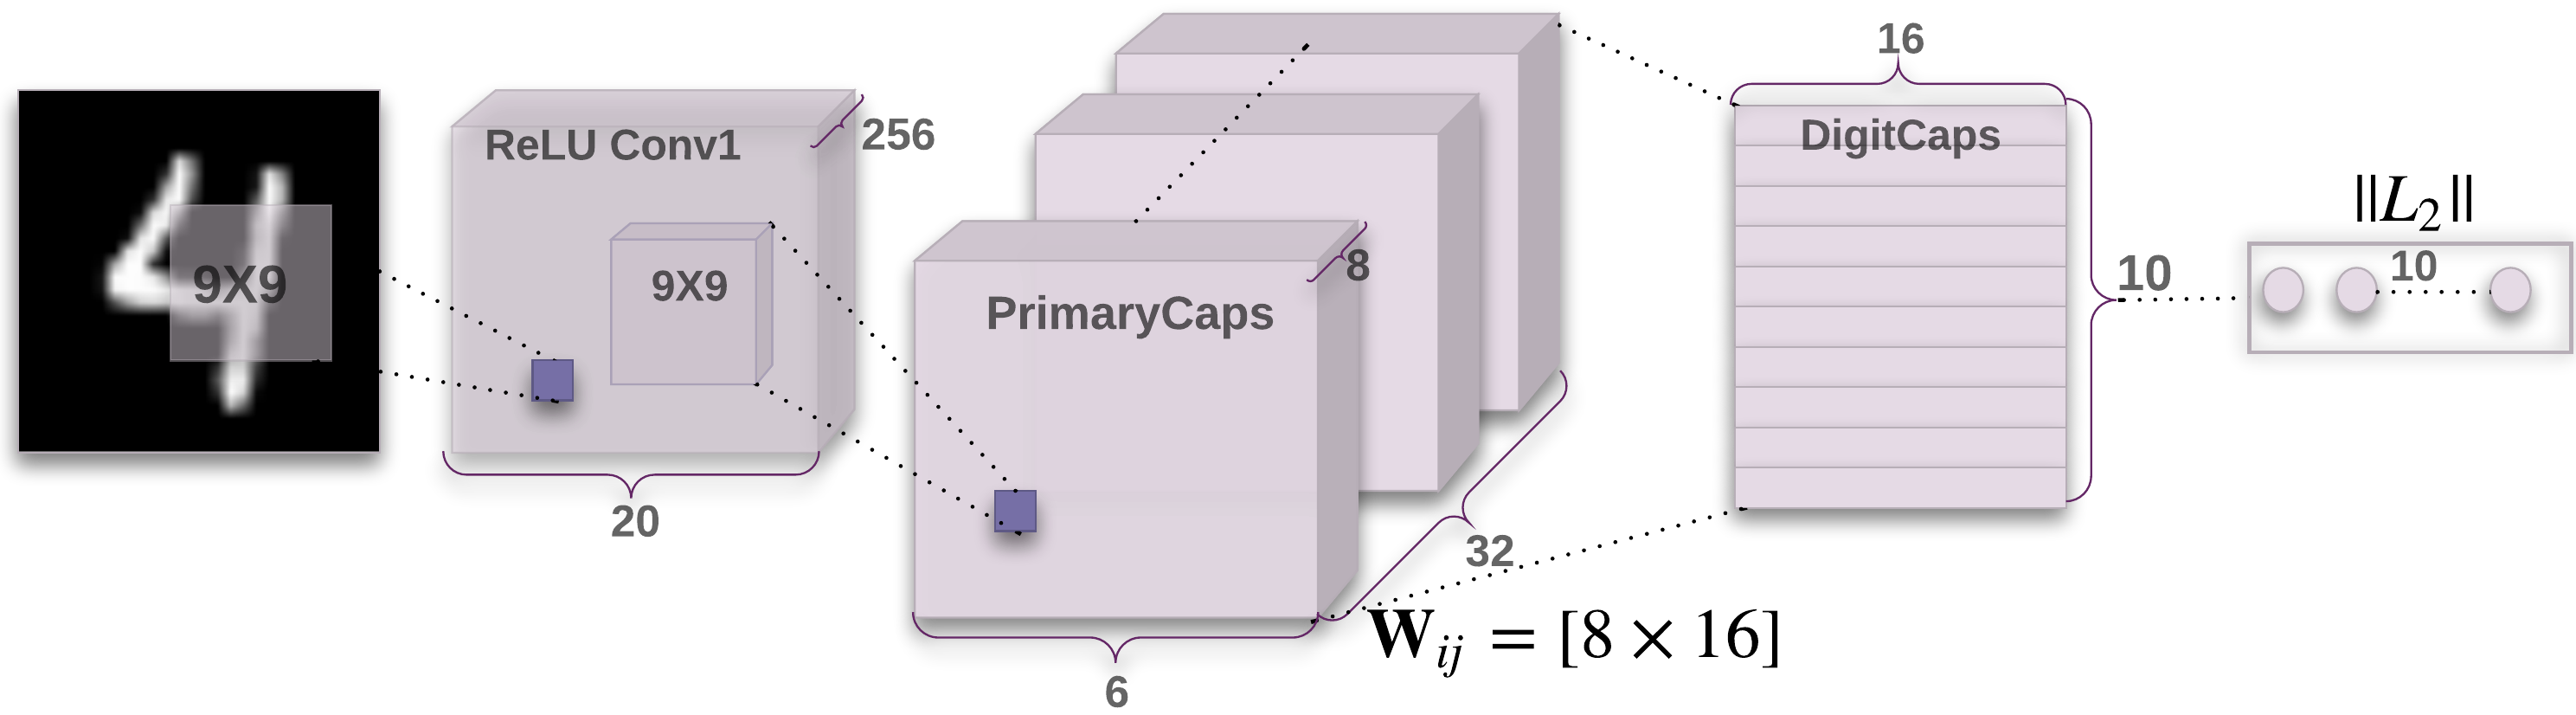
\includegraphics[width=\textwidth]{../img/capsulearch.png}
  %    \end{center}
  %  \end{frame}
  %}

  \subsection{What is a capsule?}
  {
    \setbeamertemplate{frame footer}{\colorcite\url{https://medium.com/ai³-theory-practice-business/understanding-hintons-capsule-networks-part-ii-how-capsules-work-153b6ade9f66}}

    \begin{frame}{What Is a Capsule?}
      a~group of neurons that:
      \begin{itemize}[<+- | alert@+>]
        \item perform some complicated \textbf{internal computations} on their inputs
        \item encapsulate their results into a~\textbf{small vector} of highly informative outputs
        \item recognize an implicitly defined visual entity (over a~limited domain of~viewing conditions and deformations)
        \item encode the \textbf{probability} of the entity being present
        \item encode \textbf{instantiation parameters} \\
          {\tiny pose, lighting, deformation relative to entity's (implicitly defined) canonical version}
      \end{itemize}
    \end{frame}
  }

  {
    \setbeamertemplate{frame footer}{\colorcite\url{https://www.oreilly.com/ideas/introducing-capsule-networks}}

    \begin{frame}{Output As A Vector}
      \pause
      \begin{center}
        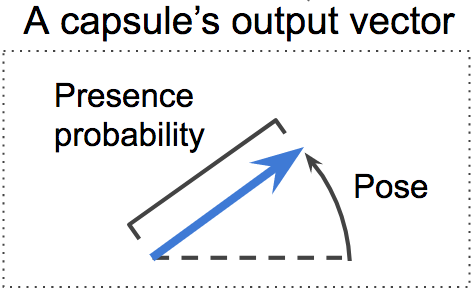
\includegraphics[height=.5\textheight]{../img/capsule-vector-output.png}
      \end{center}

      \begin{itemize}[<+- | alert@+>]
        \item probability of presence: locally \textbf{invariant} \\
          {\tiny E.g. if $0, 3, 2, 0, 0$ leads to $0, 1, 0, 0$, then $0, 0, 3, 2, 0$ should also lead to $0, 1, 0, 0$.}
        \item instantiation parameters: \textbf{equivariant} \\
          {\tiny E.g. if $0, 3, 2, 0, 0$ leads to $0, 1, 0, 0$, then $0, 0, 3, 2, 0$ might lead to $0, 0, 1, 0$.}
      \end{itemize}
    \end{frame}
  }

  {
    \setbeamertemplate{frame footer}{\colorcite[\cite{Hinton2011transforming}]}

    \begin{frame}{Previous Version of Capsules \\
        \tiny for illustration (``Transforming Auto-Encoders'' [\cite{Hinton2011transforming}])}
      \pause
      \begin{center}
        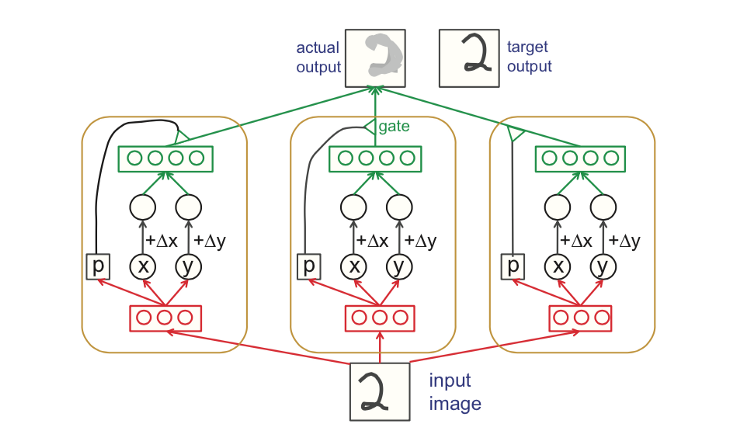
\includegraphics[width=\linewidth]{../img/transforming-auto-encoder.png}
        \tiny three capsules of a~transforming auto-encoder (that models translation)
      \end{center}
    \end{frame}
  }

  {
    \setbeamertemplate{frame footer}{\colorcite\url{https://cdn-images-1.medium.com/max/1250/1*GbmQ2X9NQoGuJ1M-EOD67g.png}}
    \setbeamercolor{background canvas}{bg=gray!65}

    \begin{frame}{Capsule's Vector Flow}
      \pause
      \begin{center}
        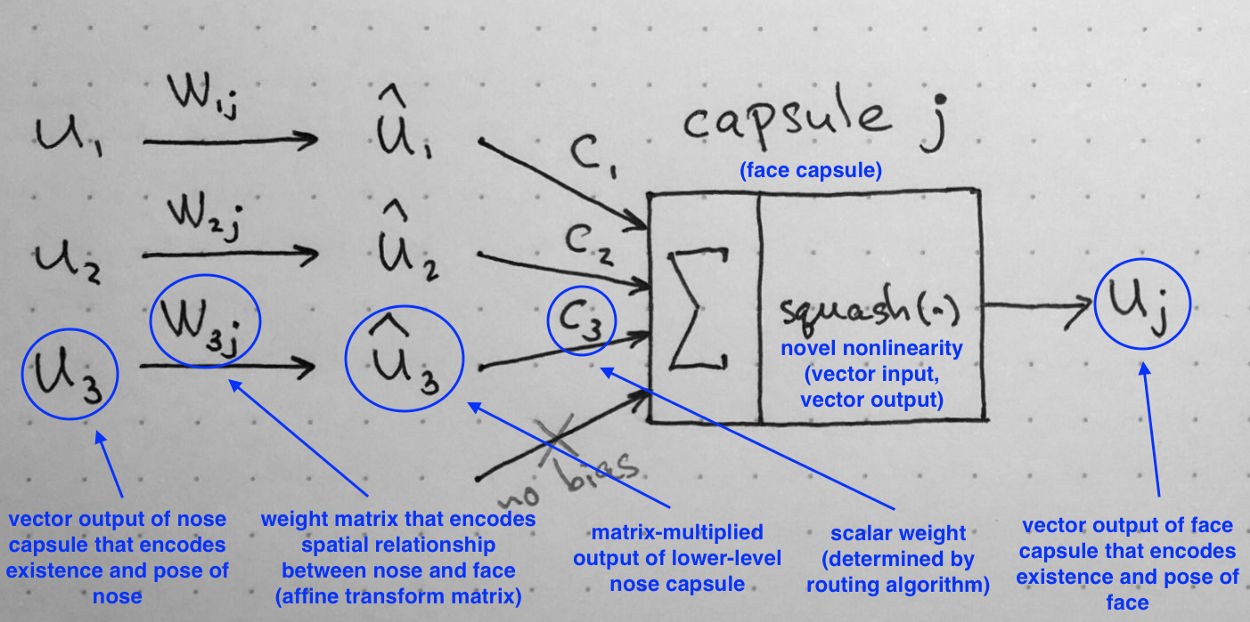
\includegraphics[width=\linewidth]{../img/capsule-pipeline.png}
        \pause
        \tiny
        \color{white}
        Note: no bias (included in affine transformation matrices $W_{ij}$'s)
      \end{center}
    \end{frame}
  }

  {
    \setbeamertemplate{frame footer}{\colorcite\url{https://github.com/naturomics/CapsNet-Tensorflow}}

    \usebackgroundtemplate{
      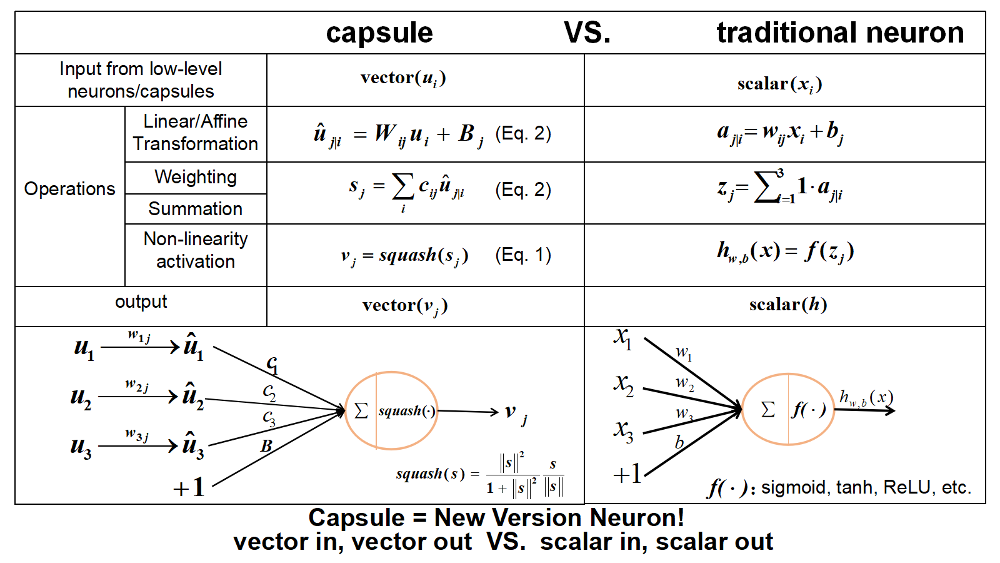
\includegraphics[width=\paperwidth]{../img/capsuleVSneuron.png}
    }
    \begin{frame}[standout]
    \end{frame}
  }

%%%%%%%%%%%%%%%%%%%%%%%%%%%%%%%%%%%%%%%%%%%%%%%%%%%%%%%%%%%%%%%%%%%%%%%%%%%%%%%%

  \section{Routing by an Agreement}

  \subsection{Algorithm}
  {
    \setbeamertemplate{frame footer}{\colorcite[\cite{Sabour2017dynamic}]}

    \begin{frame}{Capsule Schema with Routing}
      \begin{center}
        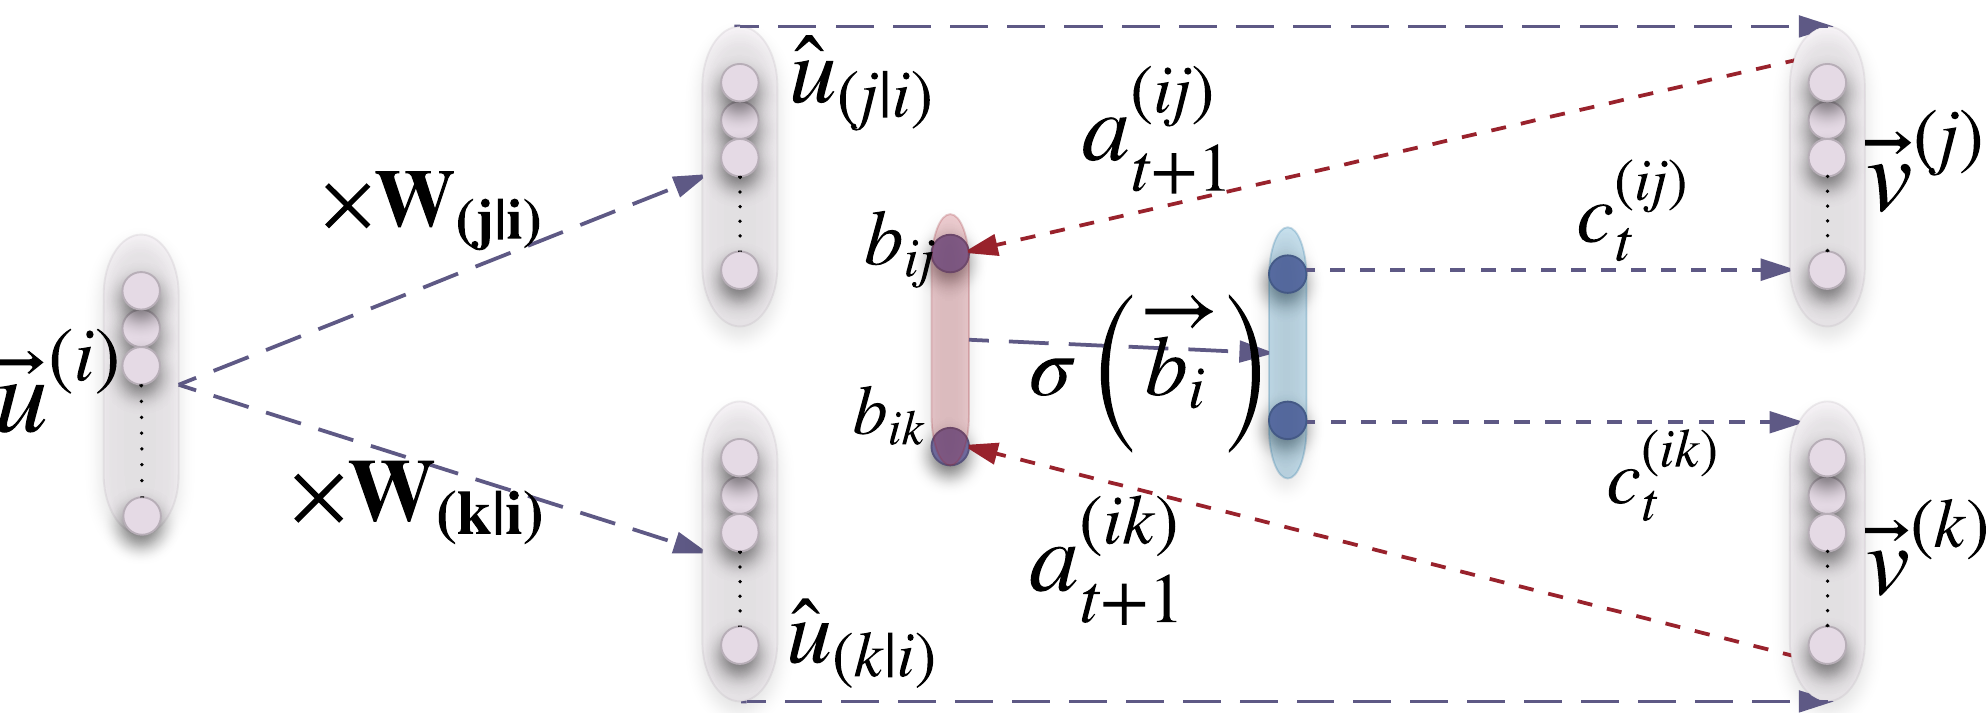
\includegraphics[width=\textwidth]{../img/capsRouting.png}
      \end{center}
    \end{frame}

    \begin{frame}{Routing Softmax}
      \begin{center}
        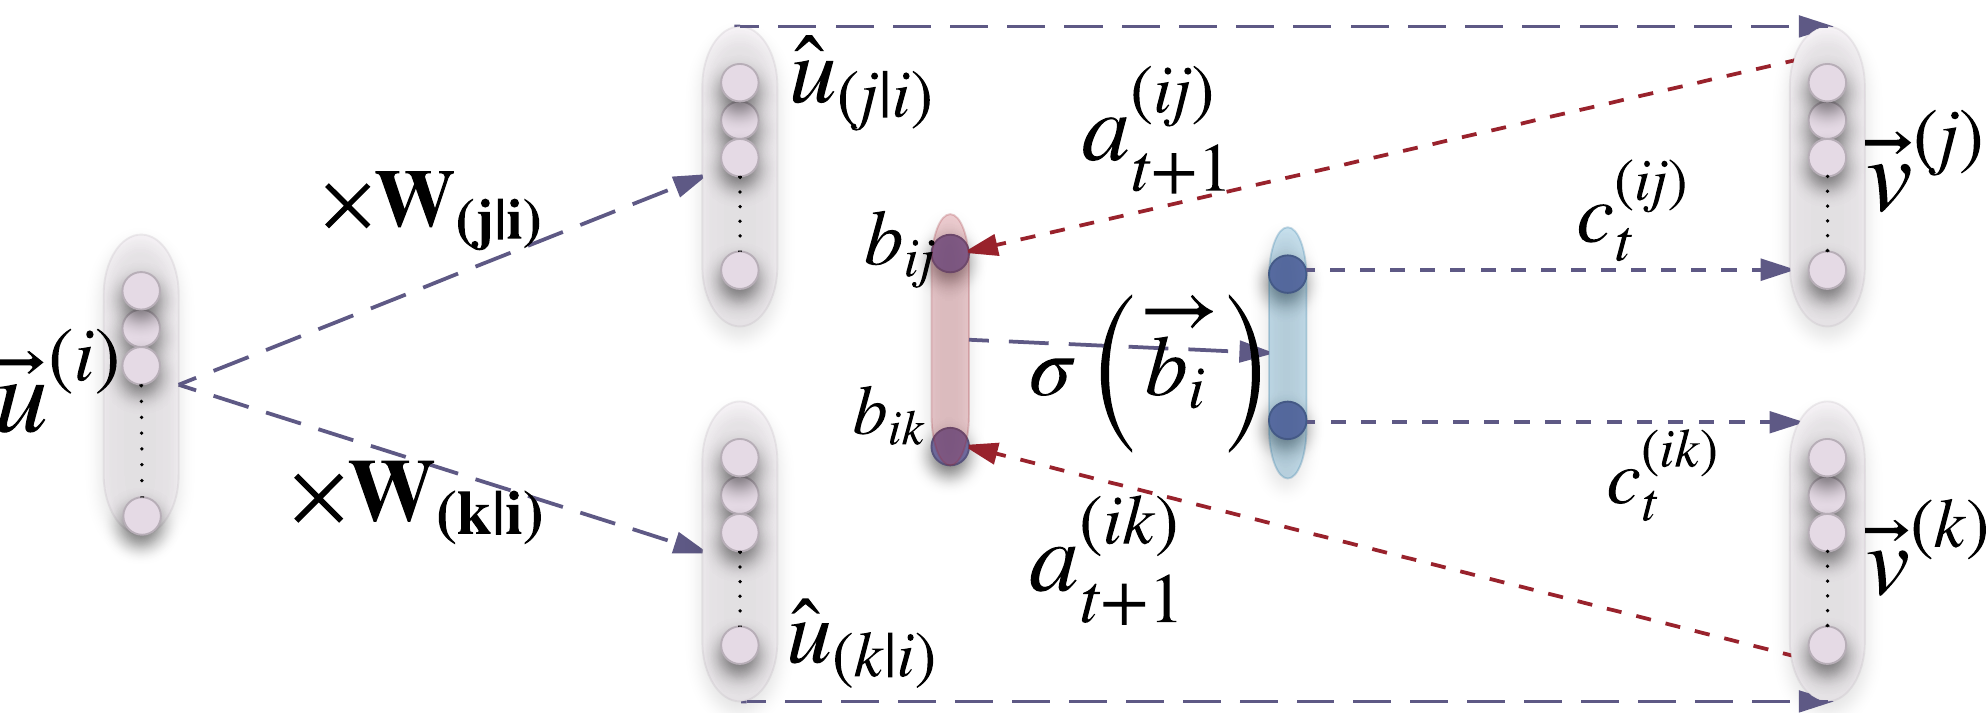
\includegraphics[width=.6\textwidth]{../img/capsRouting.png}
      \end{center}

      \begin{equation}
        c_{ij} = \frac{\exp(b_{ij})}{\sum_k \exp(b_{ik})}
        \label{eq:softmax}
      \end{equation}
    \end{frame}

    \begin{frame}{Prediction Vectors}
      \begin{center}
        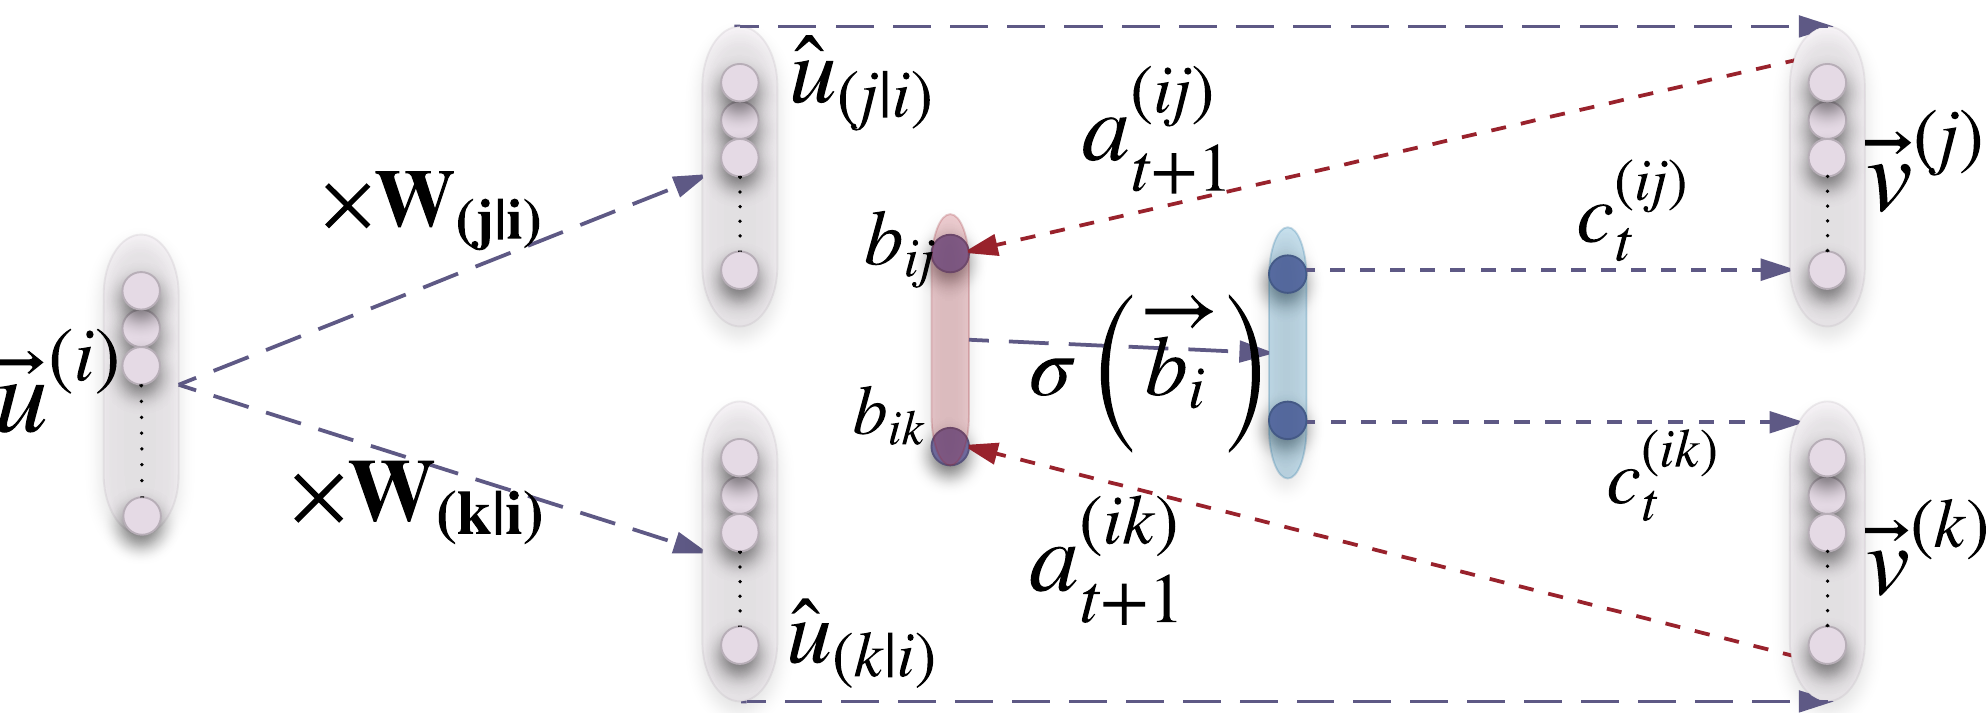
\includegraphics[width=.6\textwidth]{../img/capsRouting.png}
      \end{center}

      \begin{equation}
        {\bf \hat{u}}_{j|i} = {\bf W}_{ij}{\bf u}_i 
        \label{eq:predict-vecs}
      \end{equation}
    \end{frame}

    \begin{frame}{Total Input}
      \begin{center}
        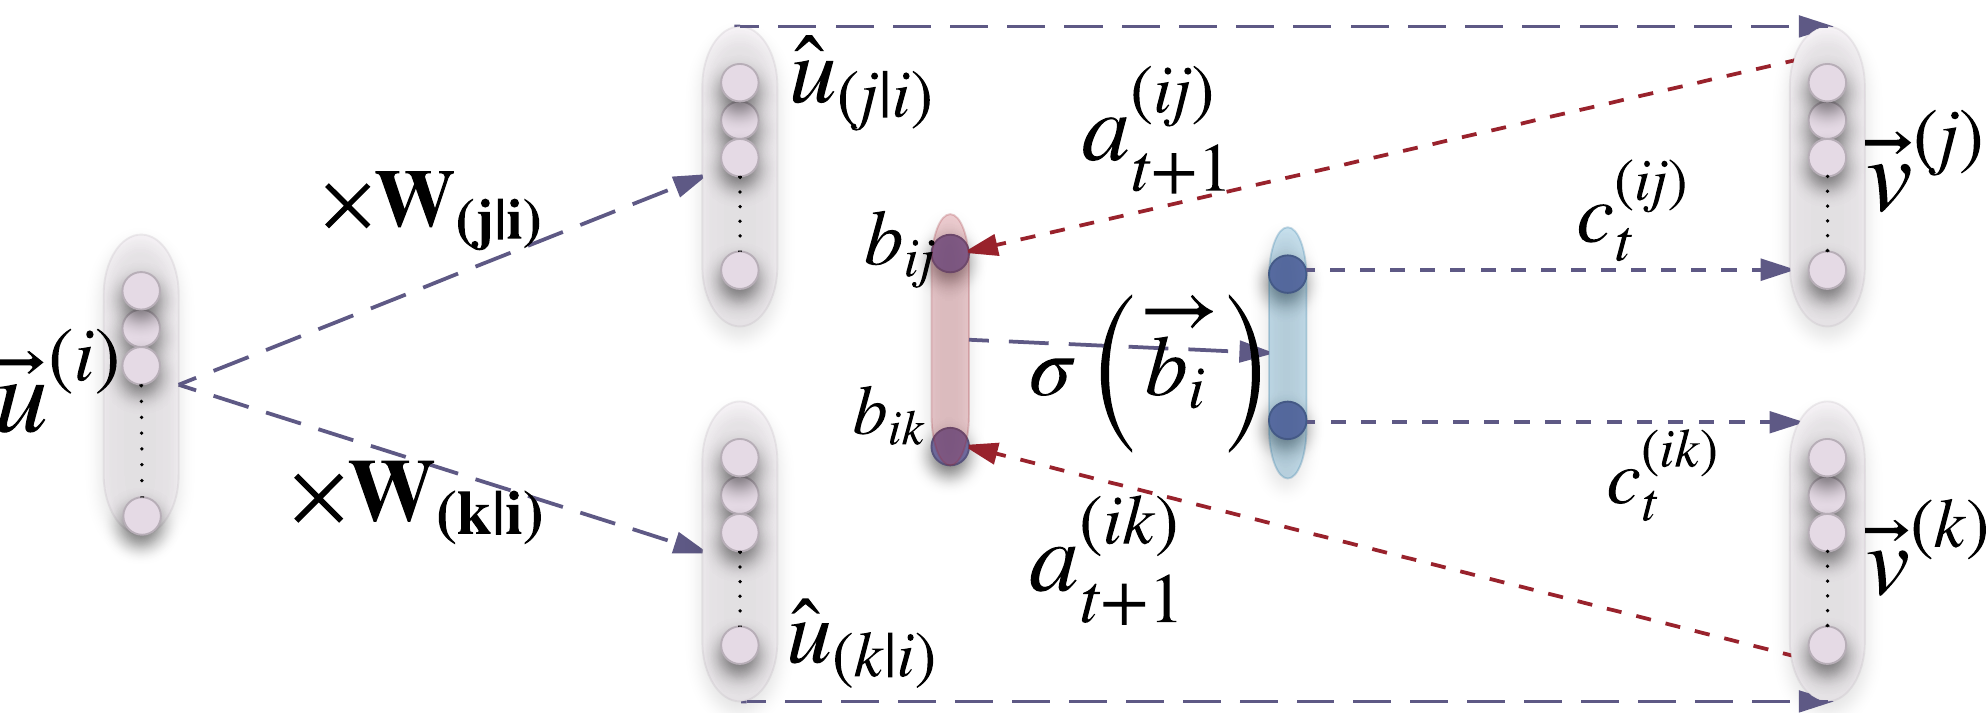
\includegraphics[width=.6\textwidth]{../img/capsRouting.png}
      \end{center}

      \begin{equation}
        {\bf s}_j = \sum_i c_{ij} {\bf \hat{u}}_{j|i}
        \label{eq:total-input}
      \end{equation}
    \end{frame}

    \begin{frame}{Squashing: (vector) non-linearity}
      \begin{center}
        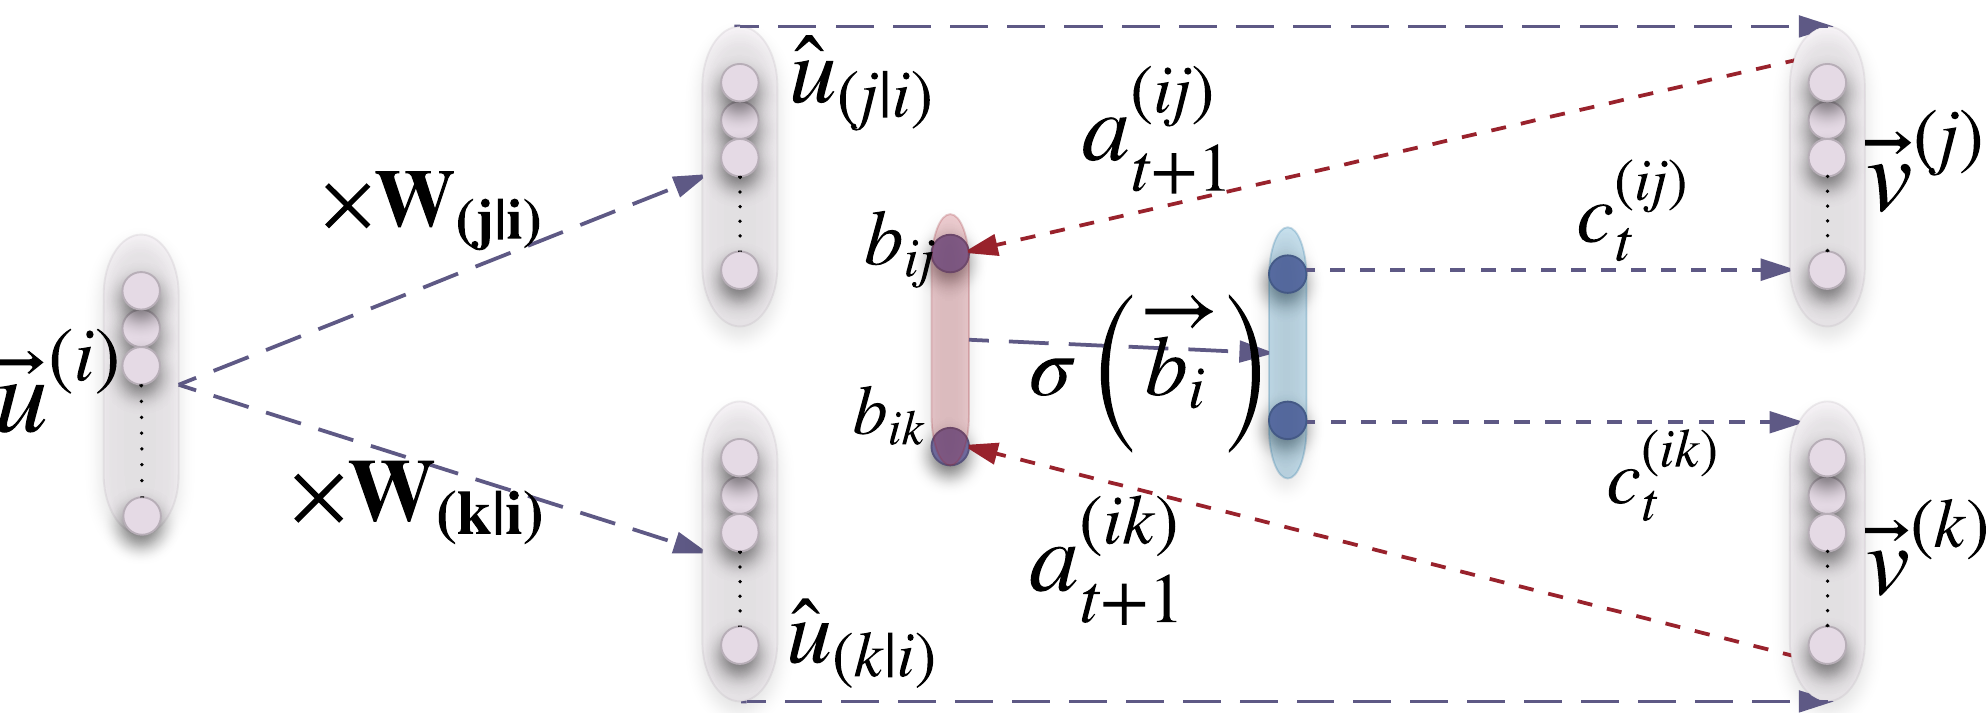
\includegraphics[width=.6\textwidth]{../img/capsRouting.png}
      \end{center}

      \begin{equation}
        {\bf v}_j = \frac{||{\bf s}_j||^2}{1+||{\bf s}_j||^2} \frac{{\bf s}_j}{||{\bf s}_j||}
        \label{eq:squash}
      \end{equation}
      \pause
    \end{frame}
  }

  {
    \setbeamertemplate{frame footer}{\colorcite\url{https://medium.com/ai³-theory-practice-business/understanding-hintons-capsule-networks-part-ii-how-capsules-work-153b6ade9f66}}
    \begin{frame}{Squashing: Plot for 1-D input}
      \begin{center}
        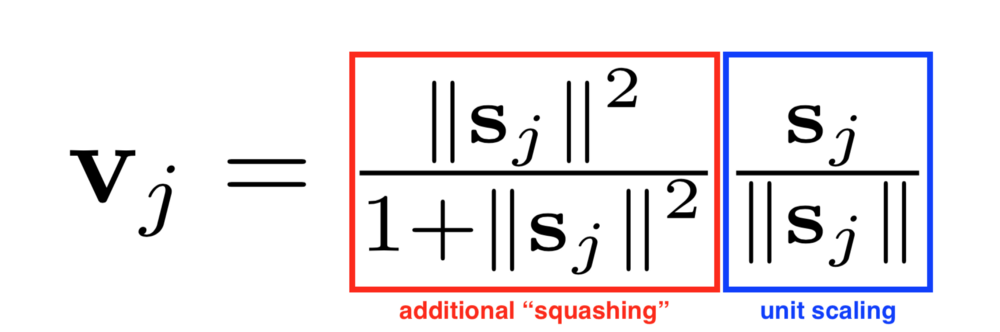
\includegraphics[width=.7\textwidth]{../img/squashing.png}
        \pause

        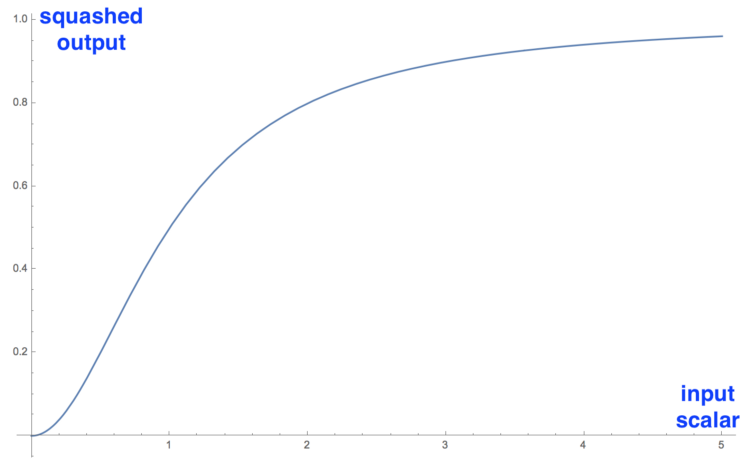
\includegraphics[width=.7\textwidth]{../img/squashing-plot.png}
      \end{center}
    \end{frame}
  }

  {
    \setbeamertemplate{frame footer}{\colorcite[\cite{Sabour2017dynamic}]}
    \begin{frame}{Routing Algorithm}
      \begin{center}
        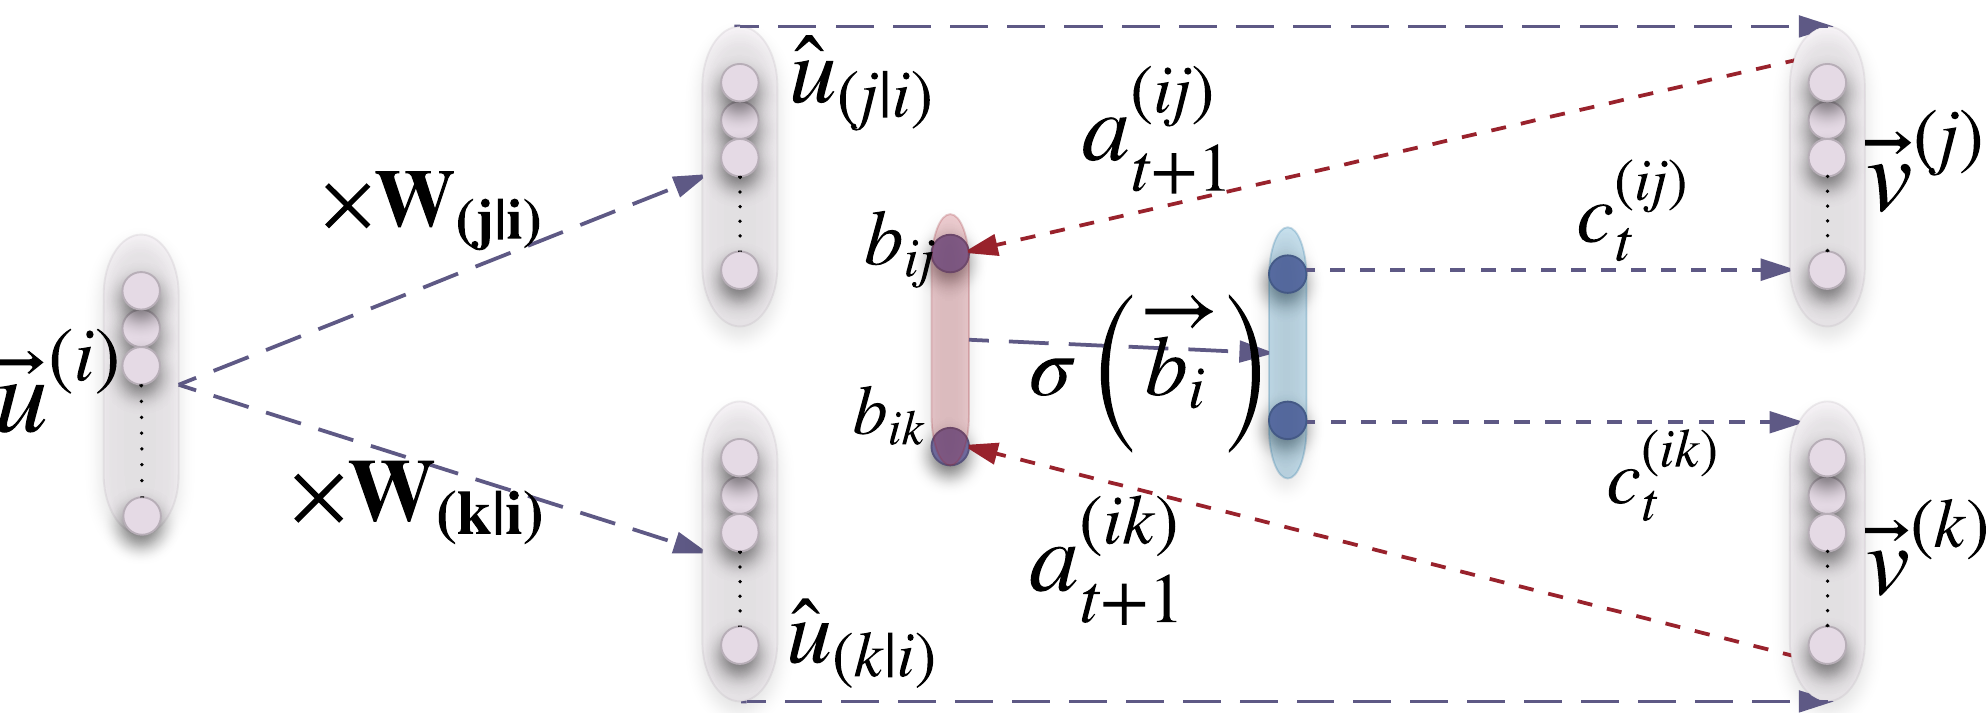
\includegraphics[width=.6\textwidth]{../img/capsRouting.png}
      \end{center}
      \pause

      \begin{algorithm}[H]
        \caption{Dynamic Routing between Capsules}
        \scriptsize
        \begin{algorithmic}[1]
          \Procedure{Routing}{$\bm{\hat{u}}_{j|i}$, $r$, $l$}
          \pause
          \State for all capsule $i$ in layer $l$ and capsule $j$ in layer $(l+1)$: $b_{ij} \gets 0$.
          \pause
          \For{$r$ iterations}
          \pause
          \State for all capsule $i$ in layer $l$: ${\bf c}_i \gets \texttt{softmax}({\bf b}_i)$ \Comment{\texttt{softmax} from Eq.~\ref{eq:softmax}}
          \pause
          \State for all capsule $j$ in layer $(l+1)$: ${\bf s}_j \gets \sum_i{c_{ij}{\bf \hat u}_{j|i}}$ \Comment{total input from Eq.~\ref{eq:total-input}}
          \pause
          \State for all capsule $j$ in layer $(l+1)$: ${\bf v}_j \gets \texttt{squash}({\bf s}_j)$ \Comment{\texttt{squash} from Eq.~\ref{eq:squash}}
          \pause
          \State for all capsule $i$ in layer $l$ and capsule $j$ in layer $(l+1)$: $b_{ij} \gets b_{ij} + {\bf \hat{u}}_{j|i} . {\bf v}_j$
          \pause
          \EndFor
          \Return ${\bf v}_j$
          \EndProcedure
        \end{algorithmic}
      \end{algorithm}
    \end{frame}
  }
  
  {
    \setbeamertemplate{frame footer}{\colorcite\url{https://youtu.be/rTawFwUvnLE?t=36m39s}}

    \usebackgroundtemplate{
      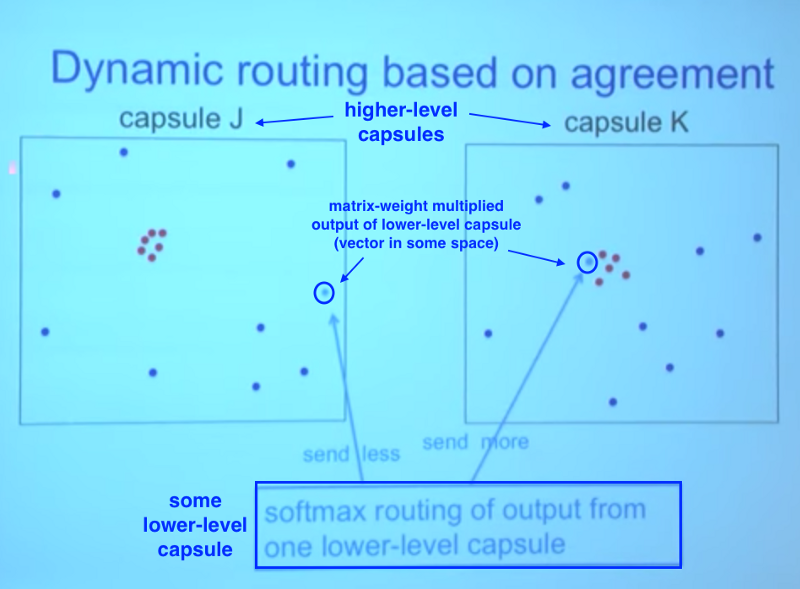
\includegraphics[height=\paperheight]{../img/hi-dim-coincidence-hinton.png}
    }
    \begin{frame}[standout]
    \end{frame}
  }

  \subsection{Routing Iterations}
  {
    \setbeamertemplate{frame footer}{\colorcite[\cite{Sabour2017dynamic}]}

    \begin{frame}{Average Change of Each Routing Logit $b_{ij}$ \\
        \tiny (by each routing iteration during training)}
      \pause
      \begin{center}
        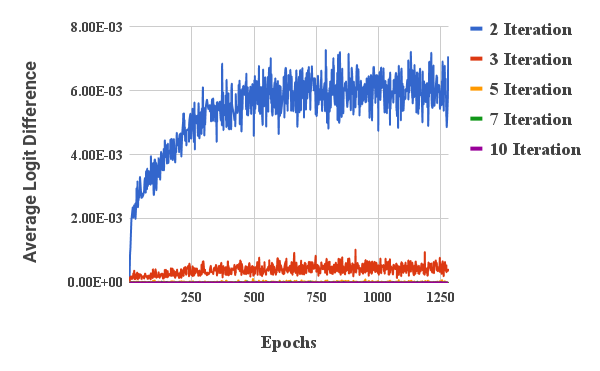
\includegraphics[width=\textwidth]{../img/conv}
      \end{center}
    \end{frame}

    \begin{frame}{Log Scale of Final Differences}
      \begin{center}
        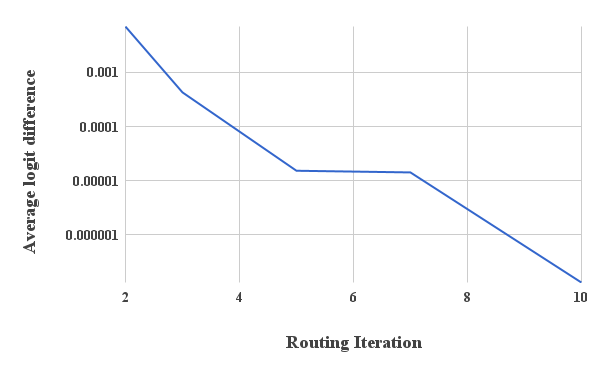
\includegraphics[width=\textwidth]{../img/c_e1}
      \end{center}
    \end{frame}


    \begin{frame}{Training Loss of CapsNet on CIFAR10 \\
        \tiny (batch size of $128$)}
      The CapsNet with \alert{$3$ routing iterations} optimizes the loss faster and converges to a~lower loss at the end.
      \pause

      \begin{center}
        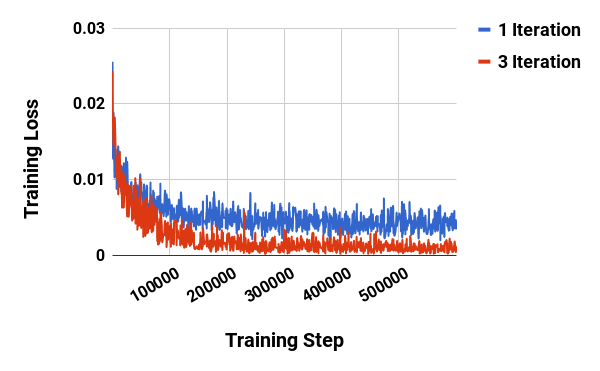
\includegraphics[width=.9\textwidth]{../img/cifar}
      \end{center}
      \pause
    \end{frame}
  }

%%%%%%%%%%%%%%%%%%%%%%%%%%%%%%%%%%%%%%%%%%%%%%%%%%%%%%%%%%%%%%%%%%%%%%%%%%%%%%%%

  \section{Capsule Network}

  {
    \setbeamertemplate{frame footer}{\colorcite[\cite{Sabour2017dynamic}]}

    \begin{frame}{Architecture: Encoder-Decoder}
      \begin{itemize}[<+- | alert@+>]
        \item encoder:
          \begin{center}
            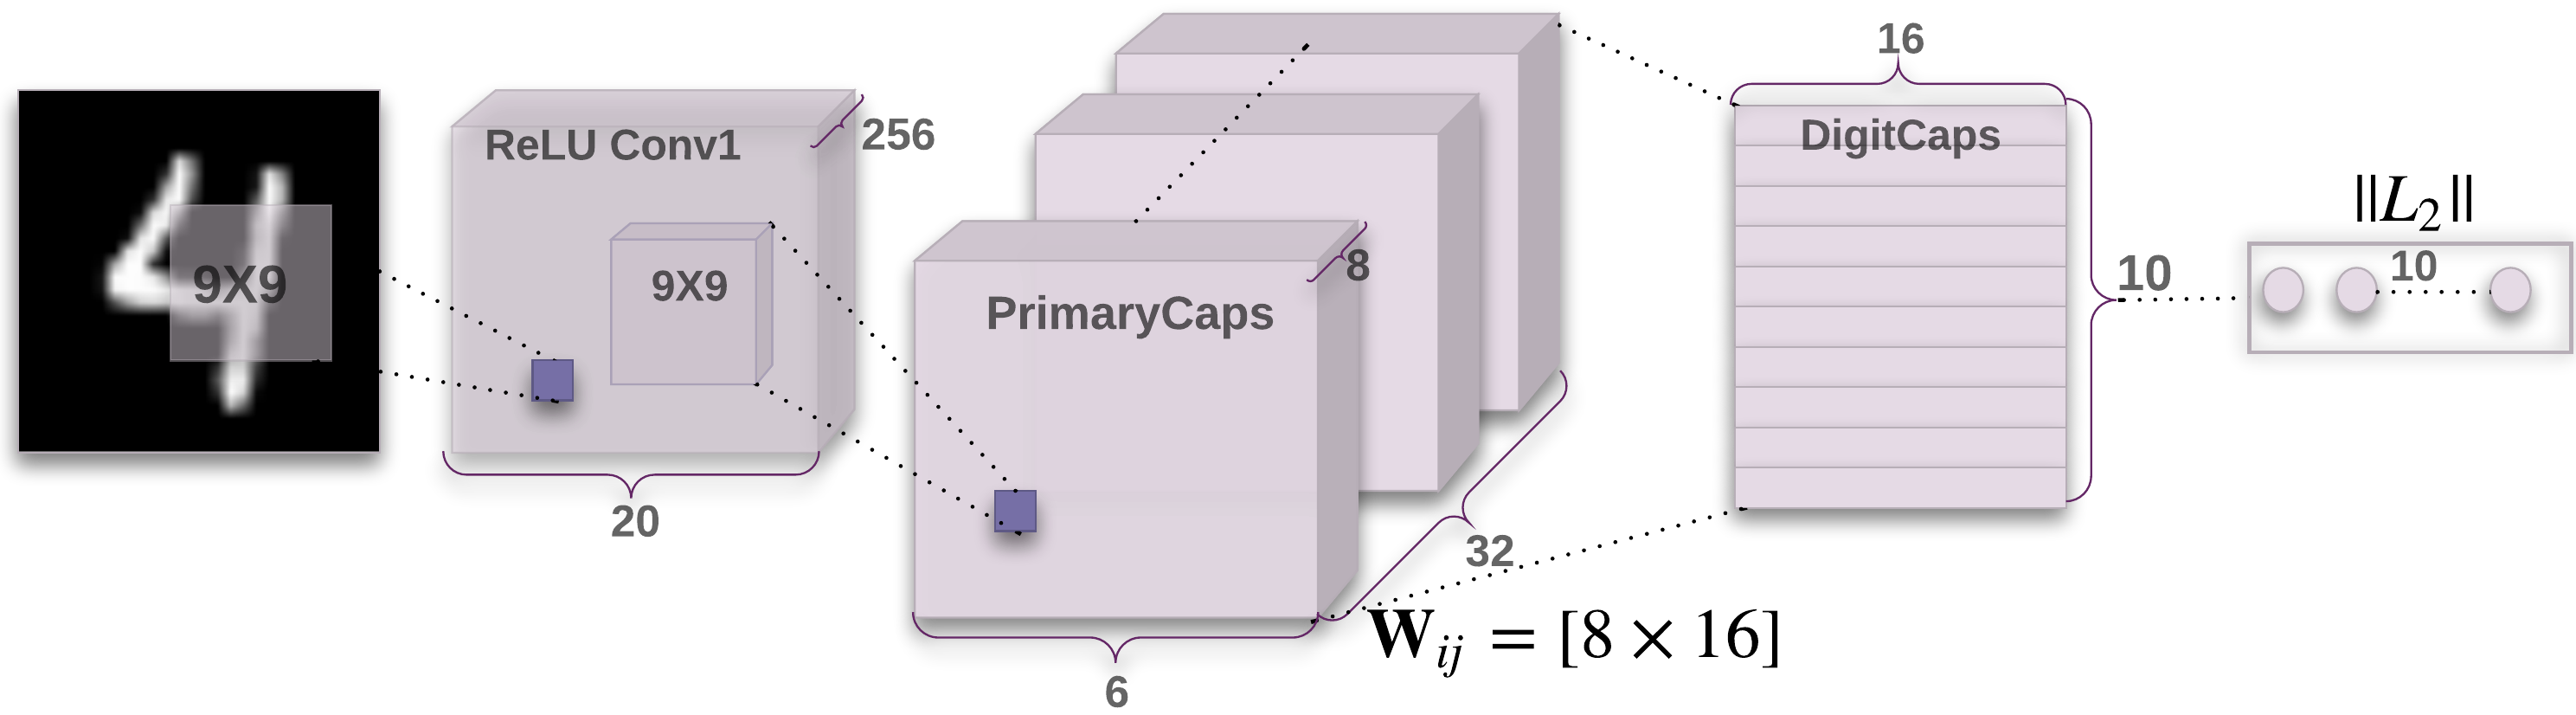
\includegraphics[width=.85\textwidth]{../img/capsulearch.png}
          \end{center}
        \item decoder:
          \begin{center}
            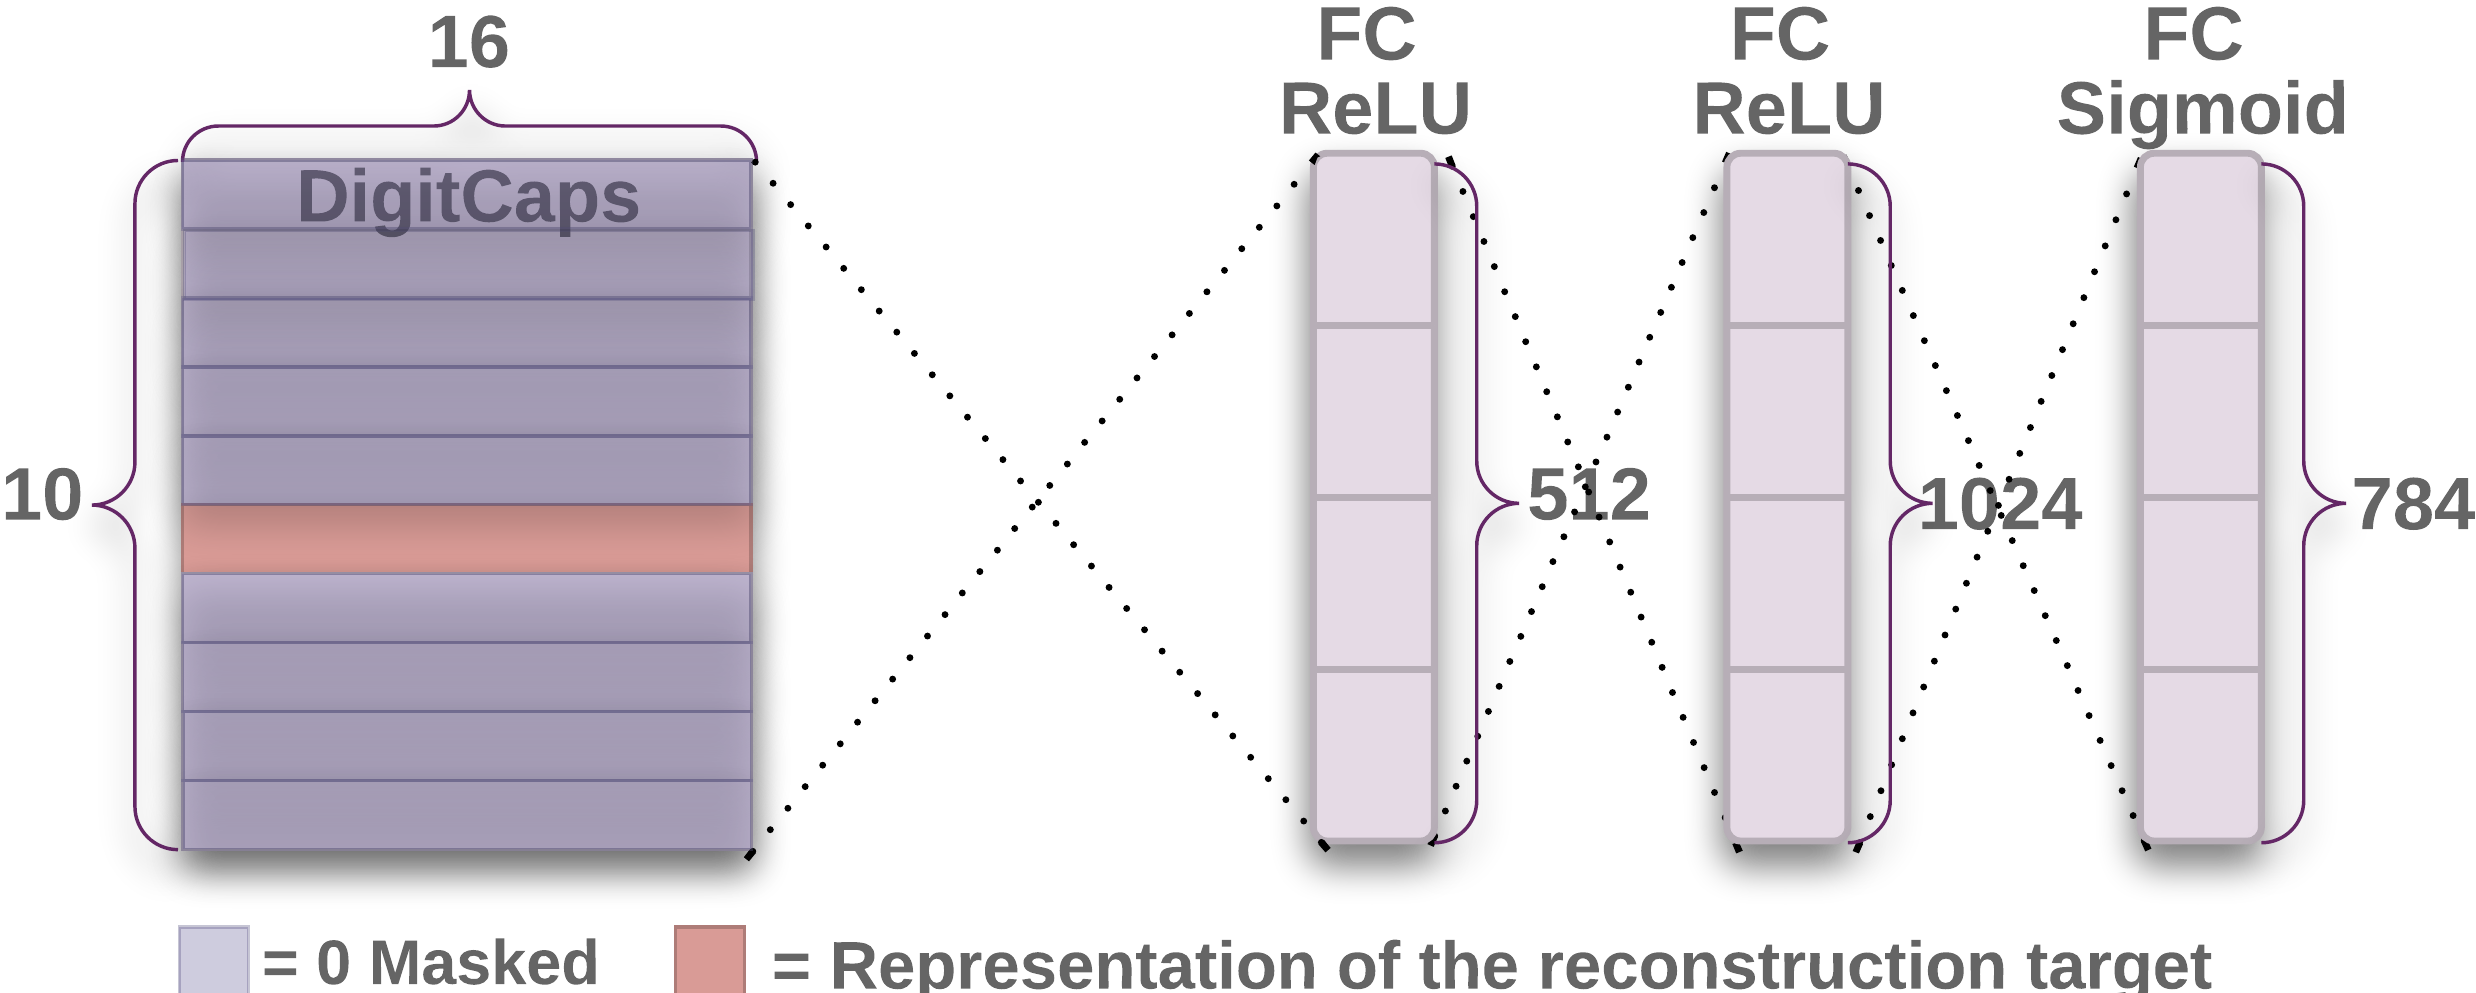
\includegraphics[width=.85\textwidth]{../img/reconsArch.png}
          \end{center}
      \end{itemize}
    \end{frame}
  }

  \subsection{Architecture: Encoder}
  {
    \setbeamertemplate{frame footer}{\colorcite[\cite{Sabour2017dynamic}]}

    \begin{frame}{Encoder: CapsNet with 3 Layers}
      \begin{center}
        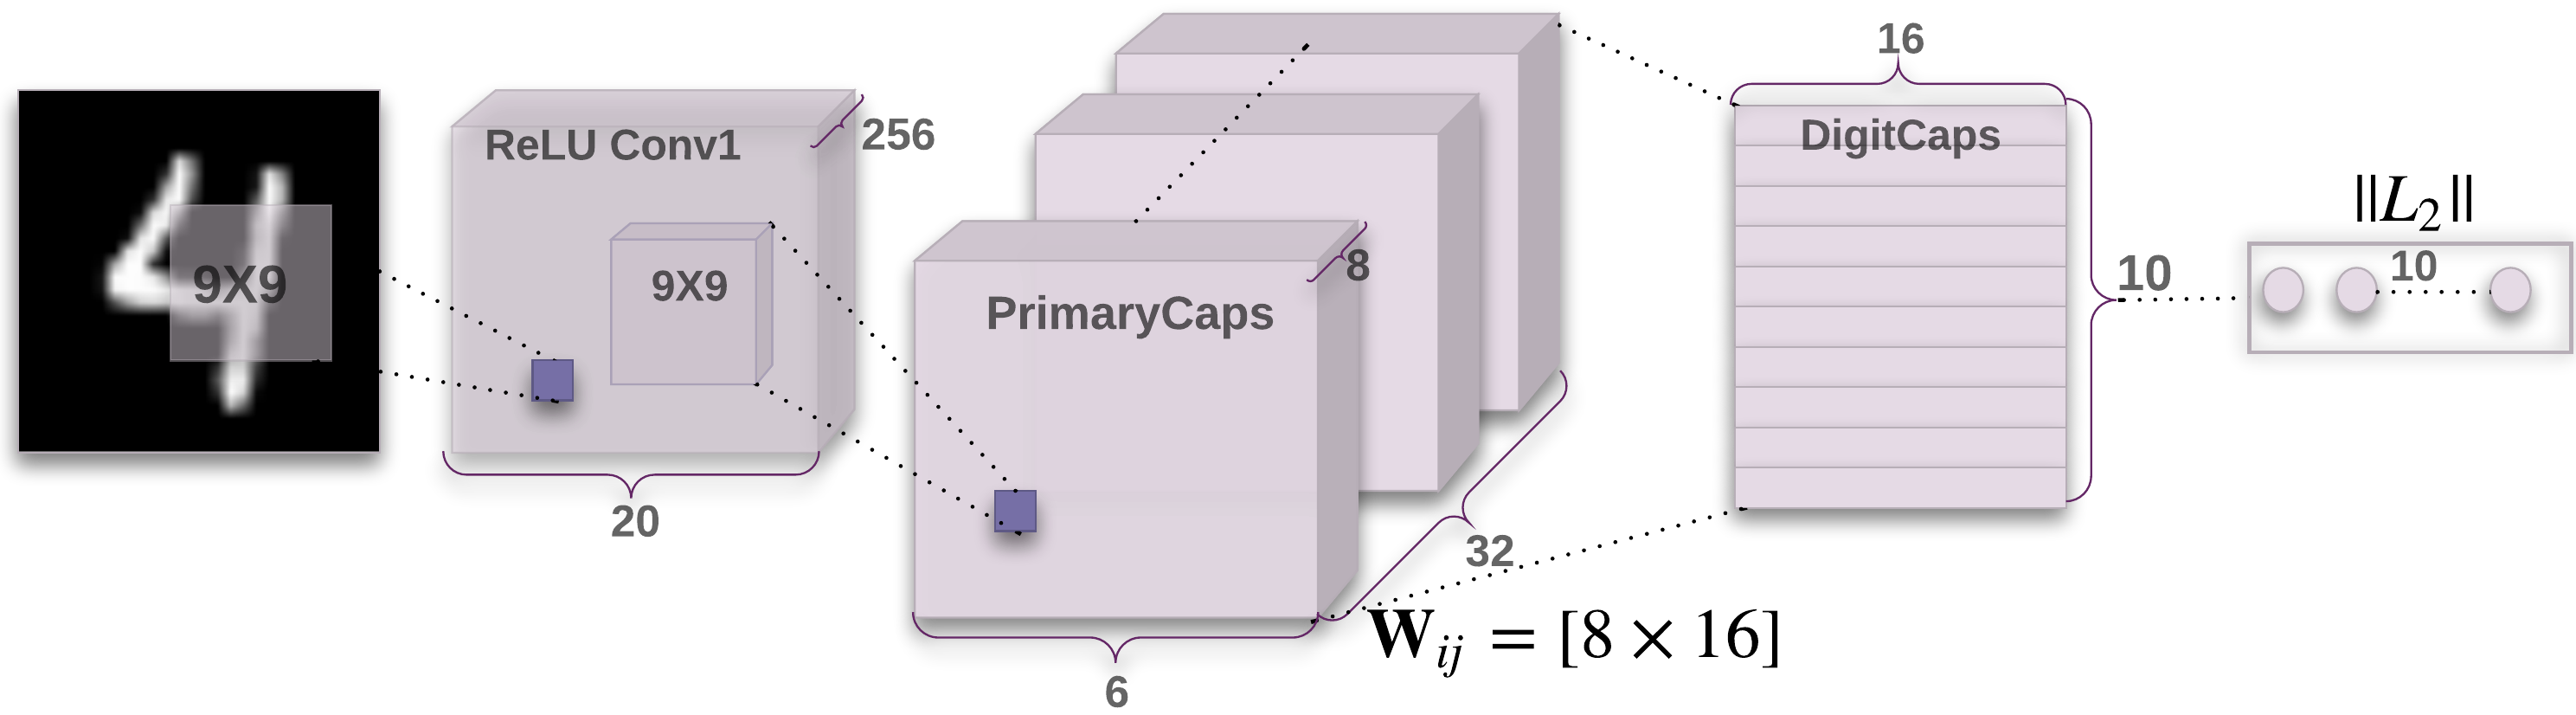
\includegraphics[width=\textwidth]{../img/capsulearch.png}
      \end{center}
      \pause

      \begin{itemize}[<+- | alert@+>]
        \item input: $28$ by $28$ MNIST digit image
        \item output: $16$-dimensional vector of instantiation parameters
      \end{itemize}
    \end{frame}

    \begin{frame}{Encoder Layer 1: (Standard) Convolutional Layer}
      \begin{center}
        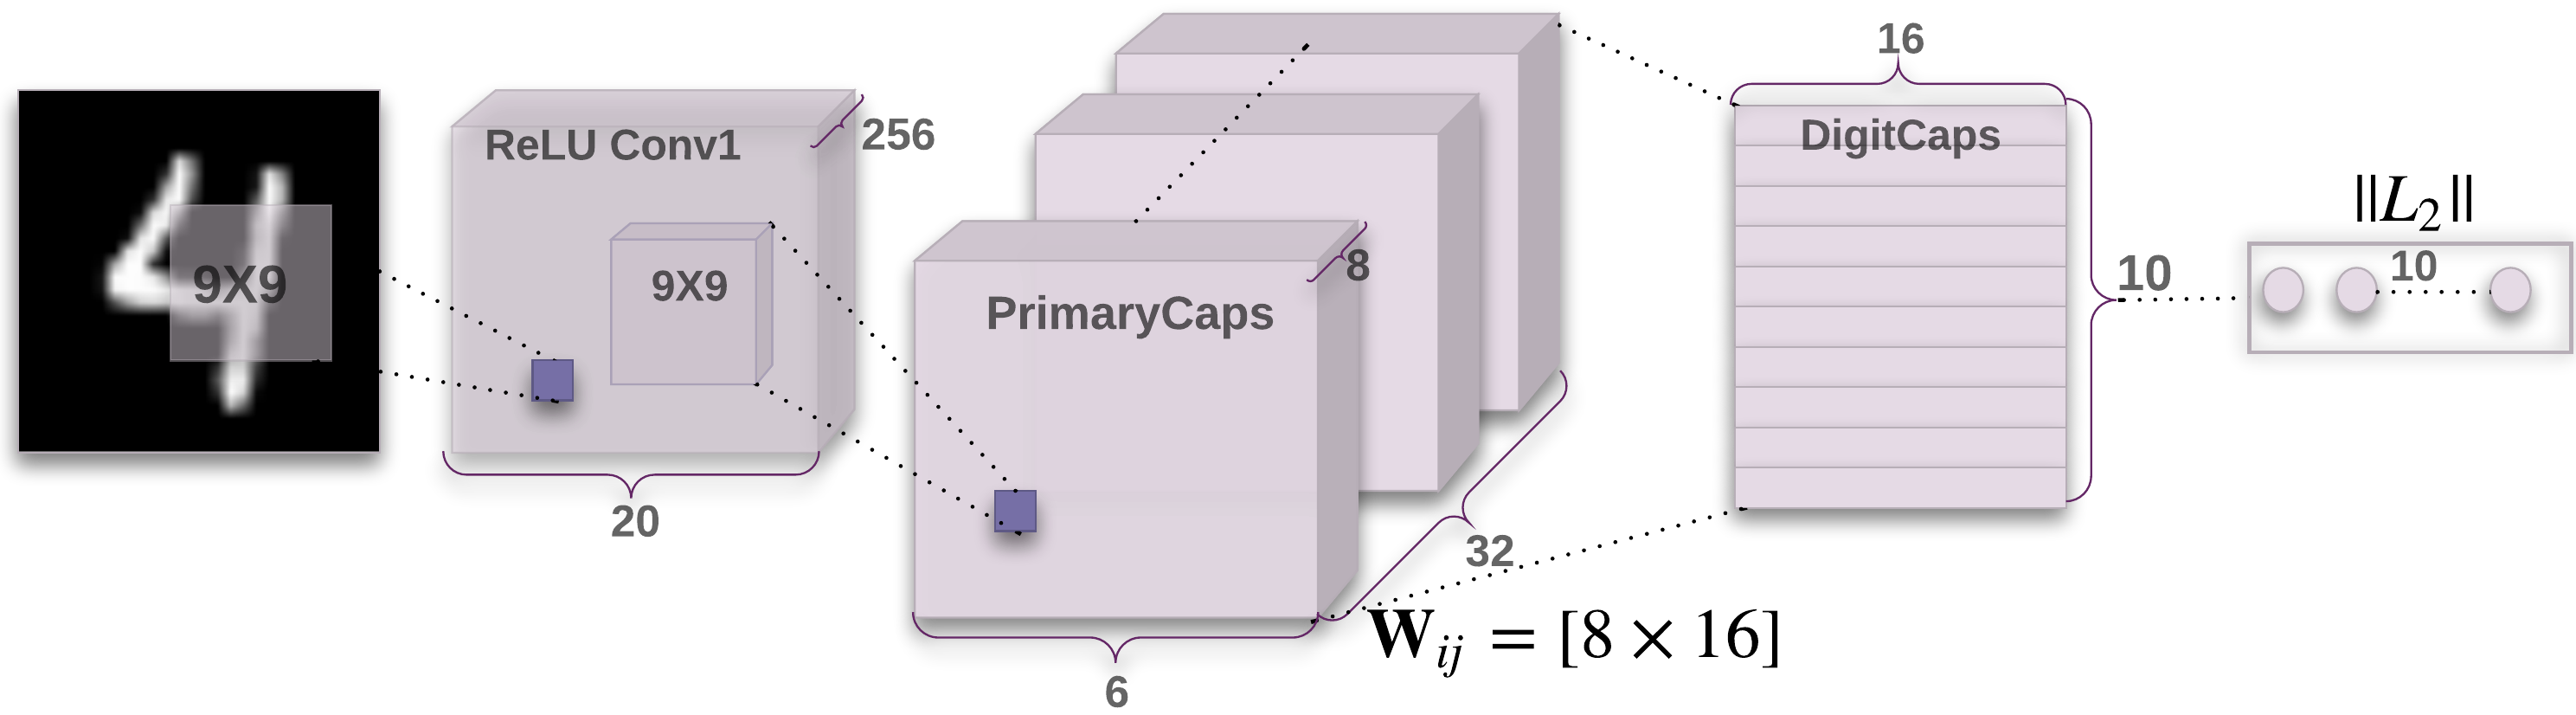
\includegraphics[width=\textwidth]{../img/capsulearch.png}
      \end{center}
      \pause

      \begin{itemize}[<+- | alert@+>]
        \item input: $28 \times 28$ image (one color channel)
        \item output: $20 \times 20 \times 256$
        \item $256$ kernels with size of $9 \times 9 \times 1$ 
        \item stride $1$
        \item ReLU activation
      \end{itemize}
    \end{frame}

    \begin{frame}{Encoder Layer 2: PrimaryCaps}
      \begin{center}
        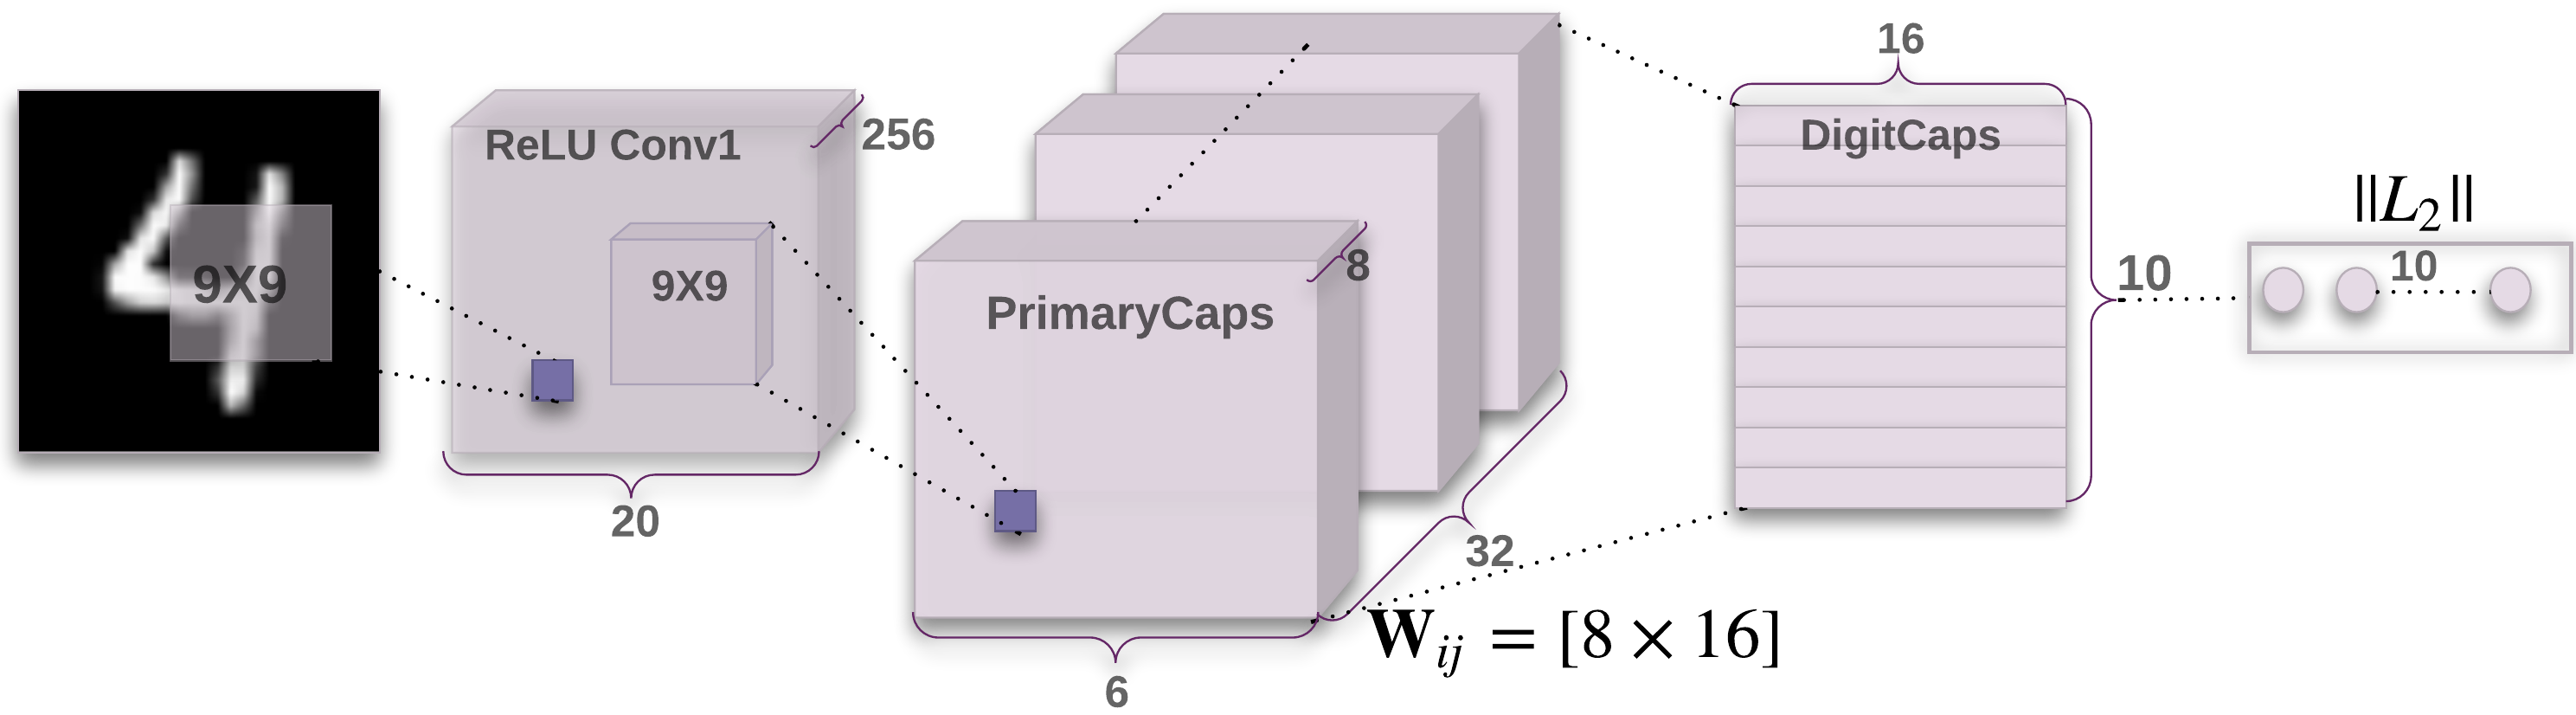
\includegraphics[width=\textwidth]{../img/capsulearch.png}
      \end{center}
      \pause

      \begin{itemize}[<+- | alert@+>]
        \item input: $20 \times 20 \times 256$ \\
          {\tiny basic features detected by the convolutional layer}
        \item output: $6 \times 6 \times 8 \times 32$ \\
          {\tiny vector (activation) outputs of primary capsules}
        \item $32$ primary capsules
        \item each applies eight $9 \times 9 \times 256$ convolutional kernels \\
          {\tiny to the $20 \times 20 \times 256$ input to produce $6 \times 6 \times 8$ output}
      \end{itemize}
    \end{frame}

    \begin{frame}{Encoder Layer 3: DigitCaps}
      \begin{center}
        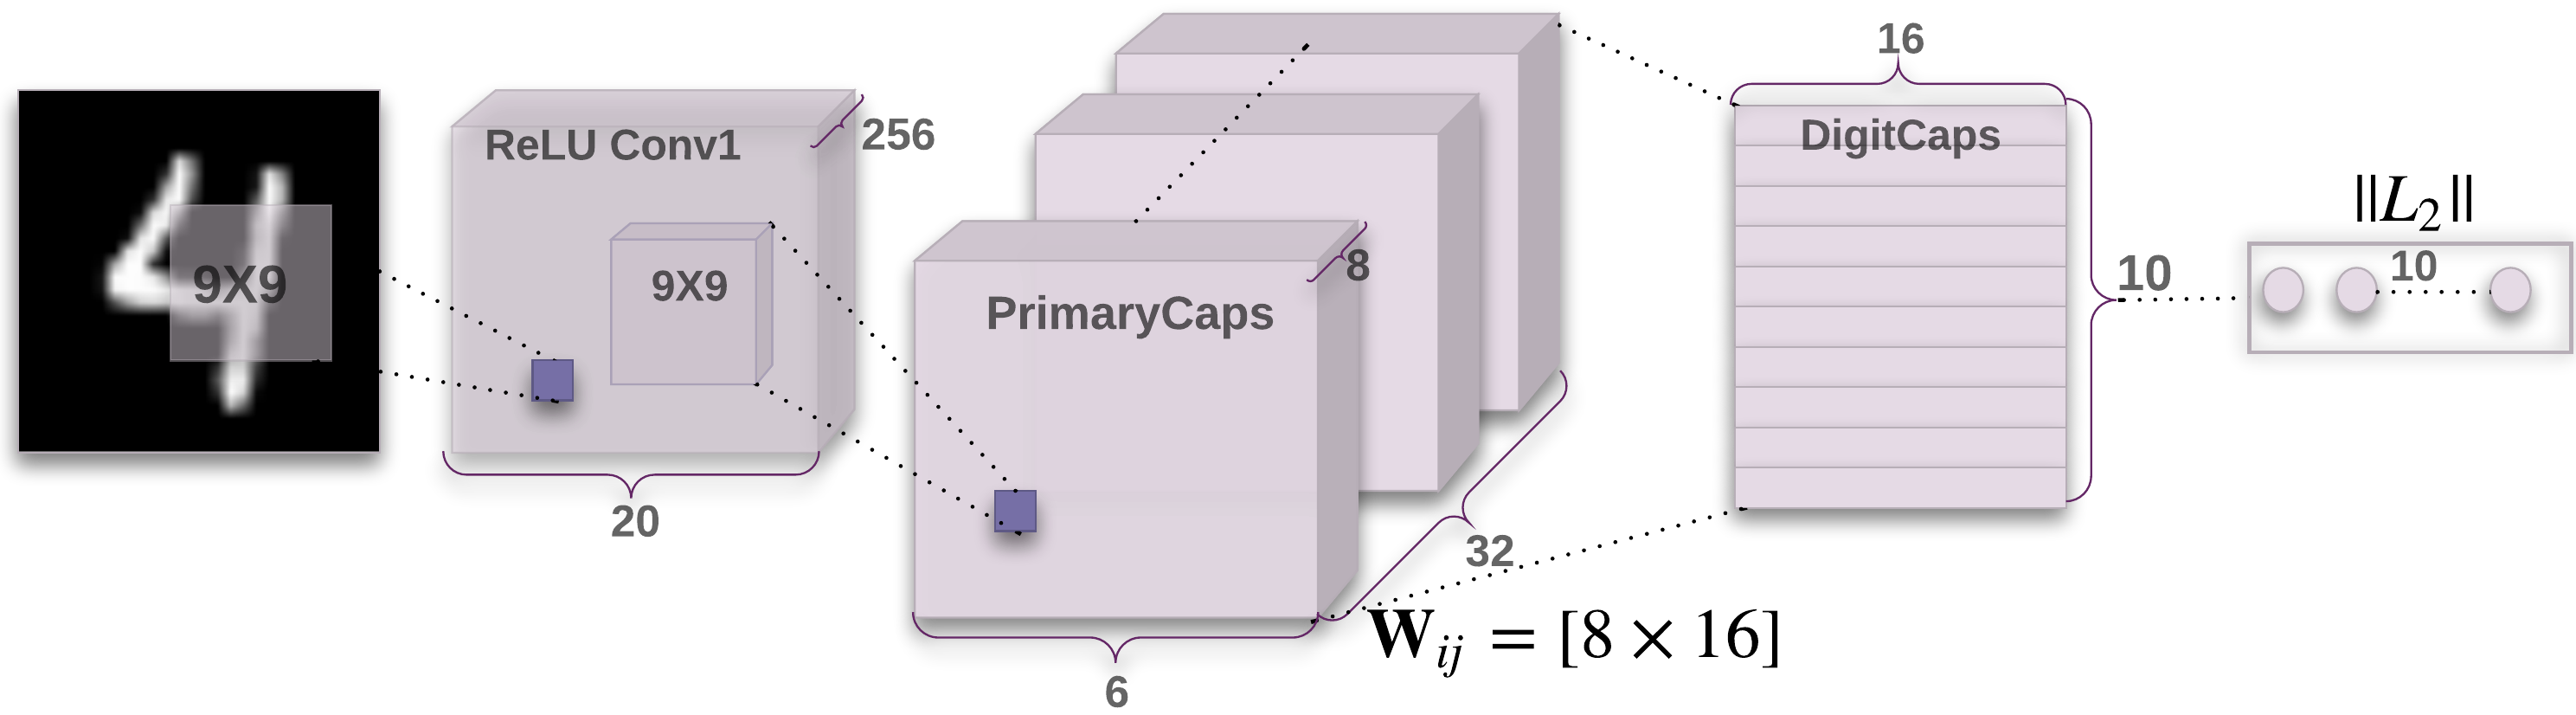
\includegraphics[width=\textwidth]{../img/capsulearch.png}
      \end{center}
      \pause

      \begin{itemize}[<+- | alert@+>]
        \item input: $6 \times 6 \times 8 \times 32$ \\
          {\tiny $(6 \times 6 \times 32)$-many $8$-dimensional vector activations}
        \item output: $16 \times 10$ \\
        \item $10$ digit capsules
        \item input vectors gets their own $8 \times 16$ weight matrix $W_{ij}$ \\
          {\tiny that maps $8$-dimensional input space to the $16$-dimensional capsule output space}
      \end{itemize}
    \end{frame}
  }

  \subsection{Loss}
  {
    \setbeamertemplate{frame footer}{\colorcite\url{https://medium.com/@pechyonkin/part-iv-capsnet-architecture-6a64422f7dce}}

    \begin{frame}{Margin Loss \\
        \tiny for a Digit Existence}
      \begin{center}
        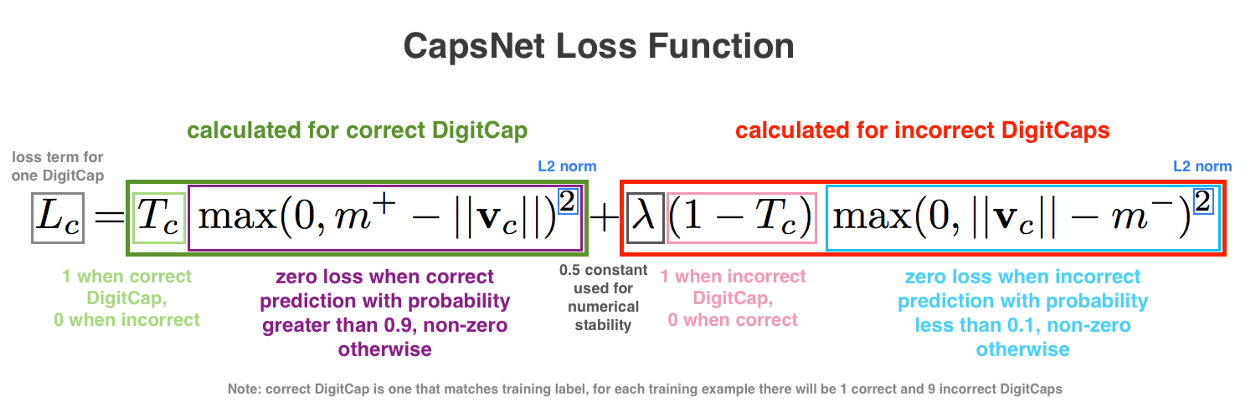
\includegraphics[width=\textwidth]{../img/capsnet-loss-details.png}
      \end{center}
    \end{frame}
  }

  {
    \setbeamertemplate{frame footer}{\colorcite[\cite{Sabour2017dynamic}]}
    \begin{frame}{Margin Loss \\
        \tiny to Train the Whole Encoder}
      In other words, each DigitCap $c$ has loss:
      \pause
      \begin{equation*}
        L_c =
        \begin{dcases*} 
          \max(0, m^{+} - ||{\bf v}_c||)^2            & iff a digit of class $c$ is present, \\
          \lambda \max(0, ||{\bf v}_c|| - m^{-})^2    & otherwise.
        \end{dcases*}
      \end{equation*}
      \pause
      \begin{itemize}[<+- | alert@+>]
        \item $m^{+} = 0.9$: \\
          {\tiny The loss is $0$ iff the \textbf{correct} DigitCap predicts the correct label with probability $\ge 0.9$.}
        \item $m^{-} = 0.1$: \\
          {\tiny The loss is $0$ iff the \textbf{mismatching} DigitCap predicts an incorrect label with probability $\le 0.1$.}
        \item $\lambda = 0.5$ is down-weighting of the loss for absent digit classes.
          {\tiny It stops the initial learning from shrinking the lengths of the activity vectors.}
        \item Squares?
          {\tiny Because there are $L_2$ norms in the loss function?}
        \item The total loss is \textbf{the sum of the losses} of all digit capsules.
      \end{itemize}
    \end{frame}
  }

  {
    \setbeamertemplate{frame footer}{\colorcite\url{https://medium.com/@pechyonkin/part-iv-capsnet-architecture-6a64422f7dce}}

    \begin{frame}{Margin Loss \\
        \tiny Function Value for Positive and for Negative Class}
      \begin{itemize}
        \item {\tiny For the \textbf{correct} DigitCap, the loss is $0$ iff it predicts the correct label with probability $\ge 0.9$.}
        \item {\tiny For the \textbf{mismatching} DigitCap, the loss is $0$ iff it predicts an incorrect label with probability $\le 0.1$.}
      \end{itemize}
      \pause

      \begin{center}
        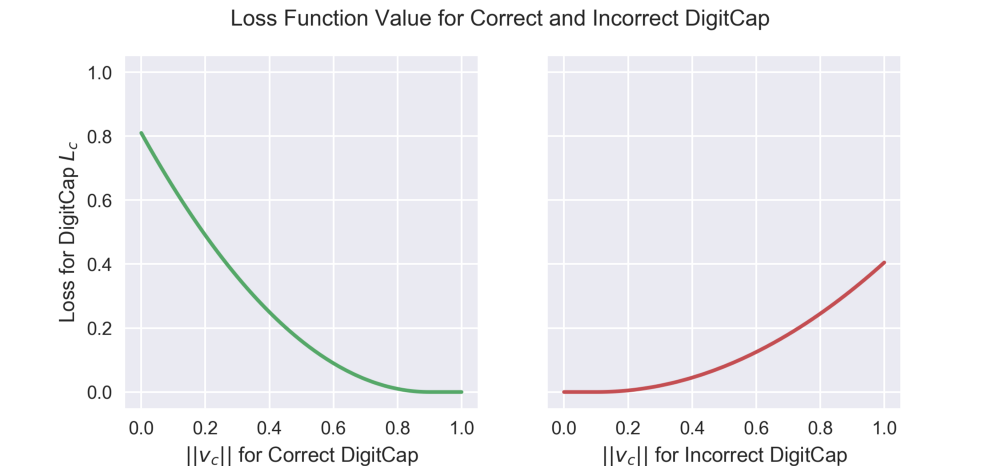
\includegraphics[width=\textwidth]{../img/capsnet-loss-plots.png}
      \end{center}
    \end{frame}
  }


  \subsection{Architecture: Decoder}
  {
    \setbeamertemplate{frame footer}{\colorcite[\cite{Sabour2017dynamic}]}

    \begin{frame}{Decoder: Regularization of CapsNets}
      \begin{center}
        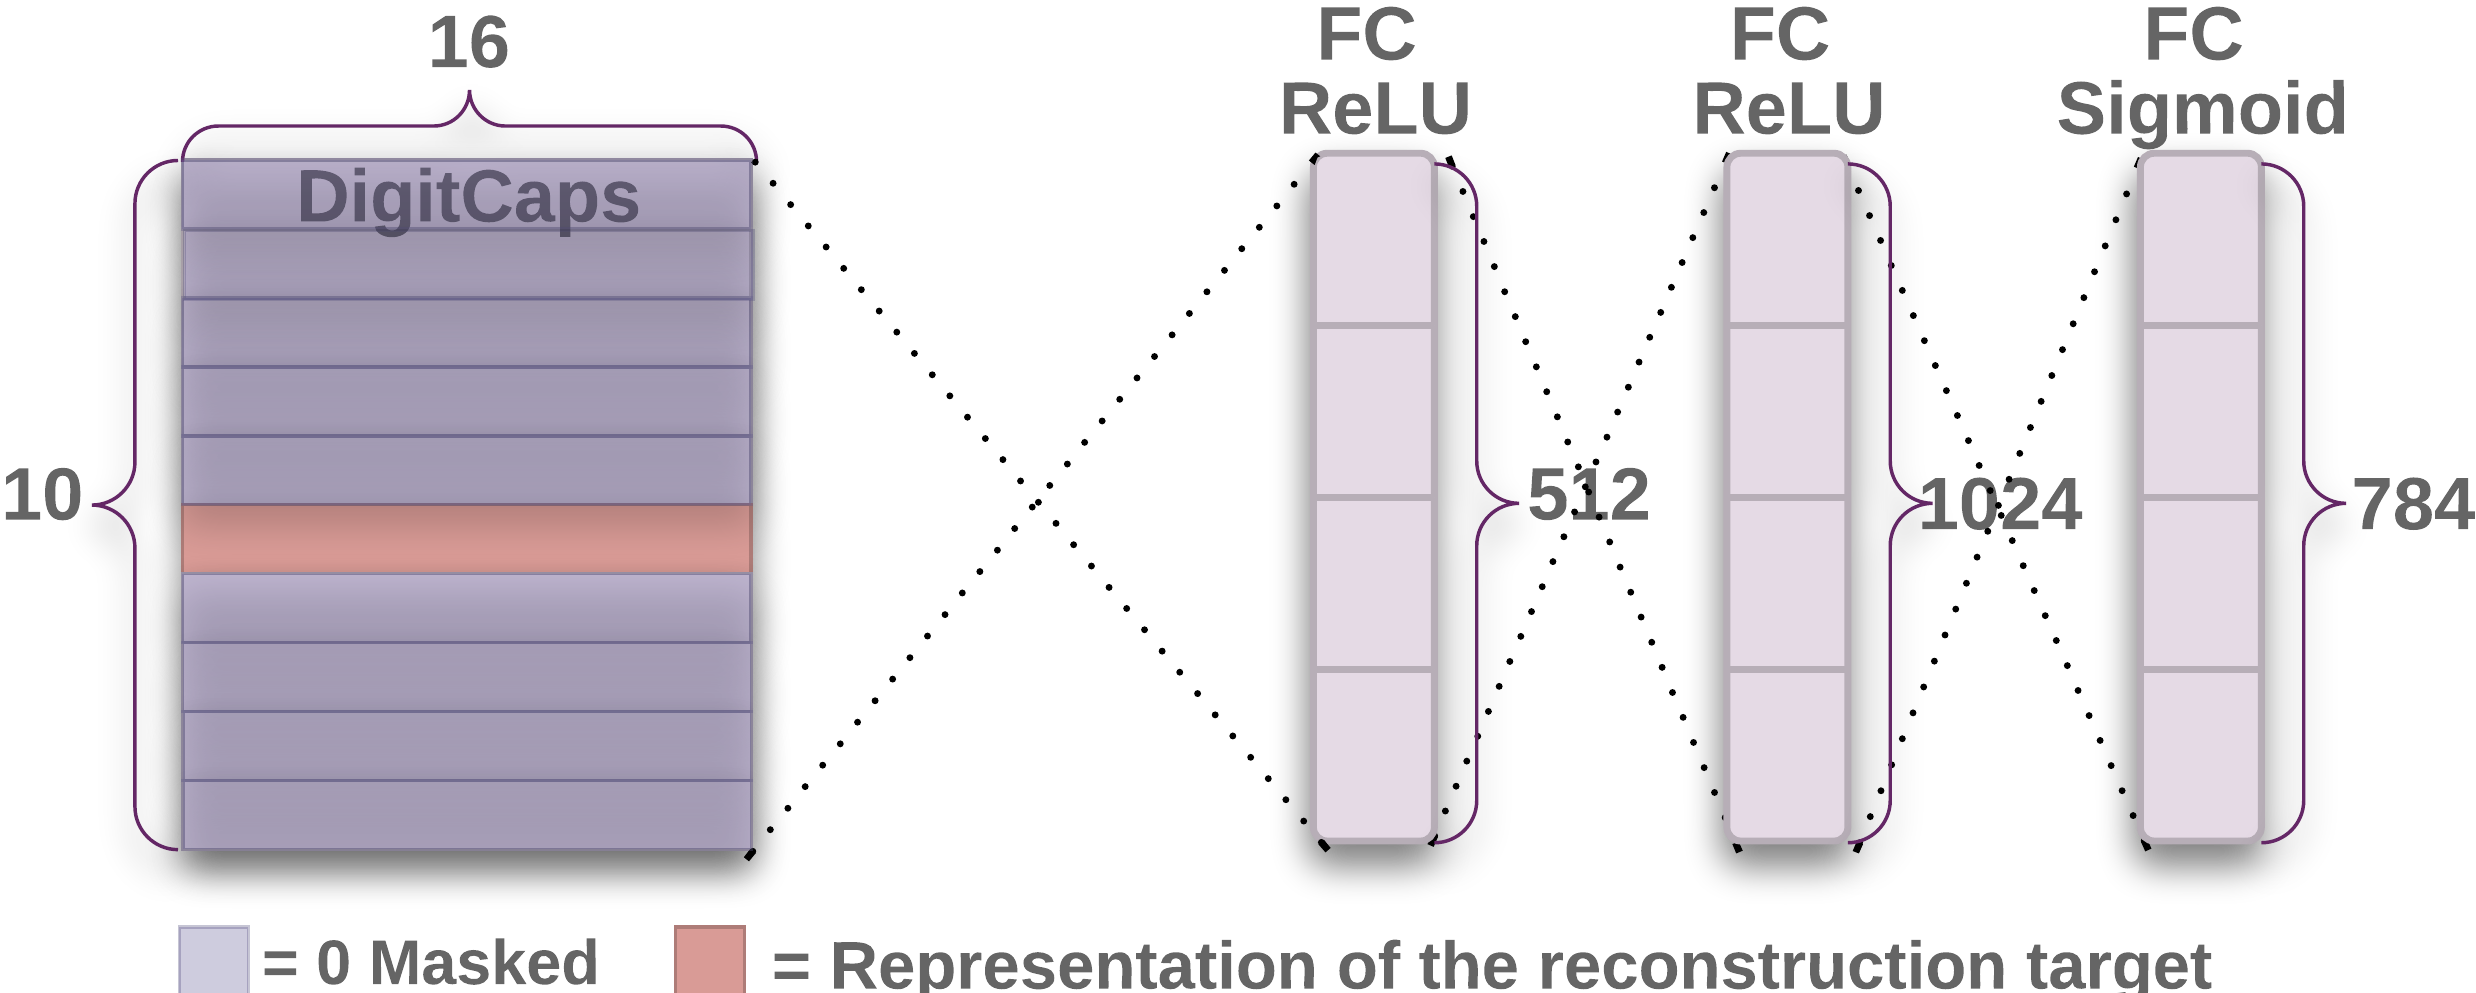
\includegraphics[width=.8\textwidth]{../img/reconsArch.png}
      \end{center}
      \pause

      Decoder is used for regularization:
      \begin{itemize}[<+- | alert@+>]
        \item decodes input from DigitCaps \\
          {\tiny to recreate an image of a $(28 \times 28)$-pixels digit}
        \item with the loss function being the Euclidean distance         % TODO -> show reconstructions
        \item ignores the negative classes
        \item forces capsules to learn features useful for reconstruction
      \end{itemize}
    \end{frame}

    \begin{frame}{Decoder: 3 Fully Connected Layers}
      \begin{center}
        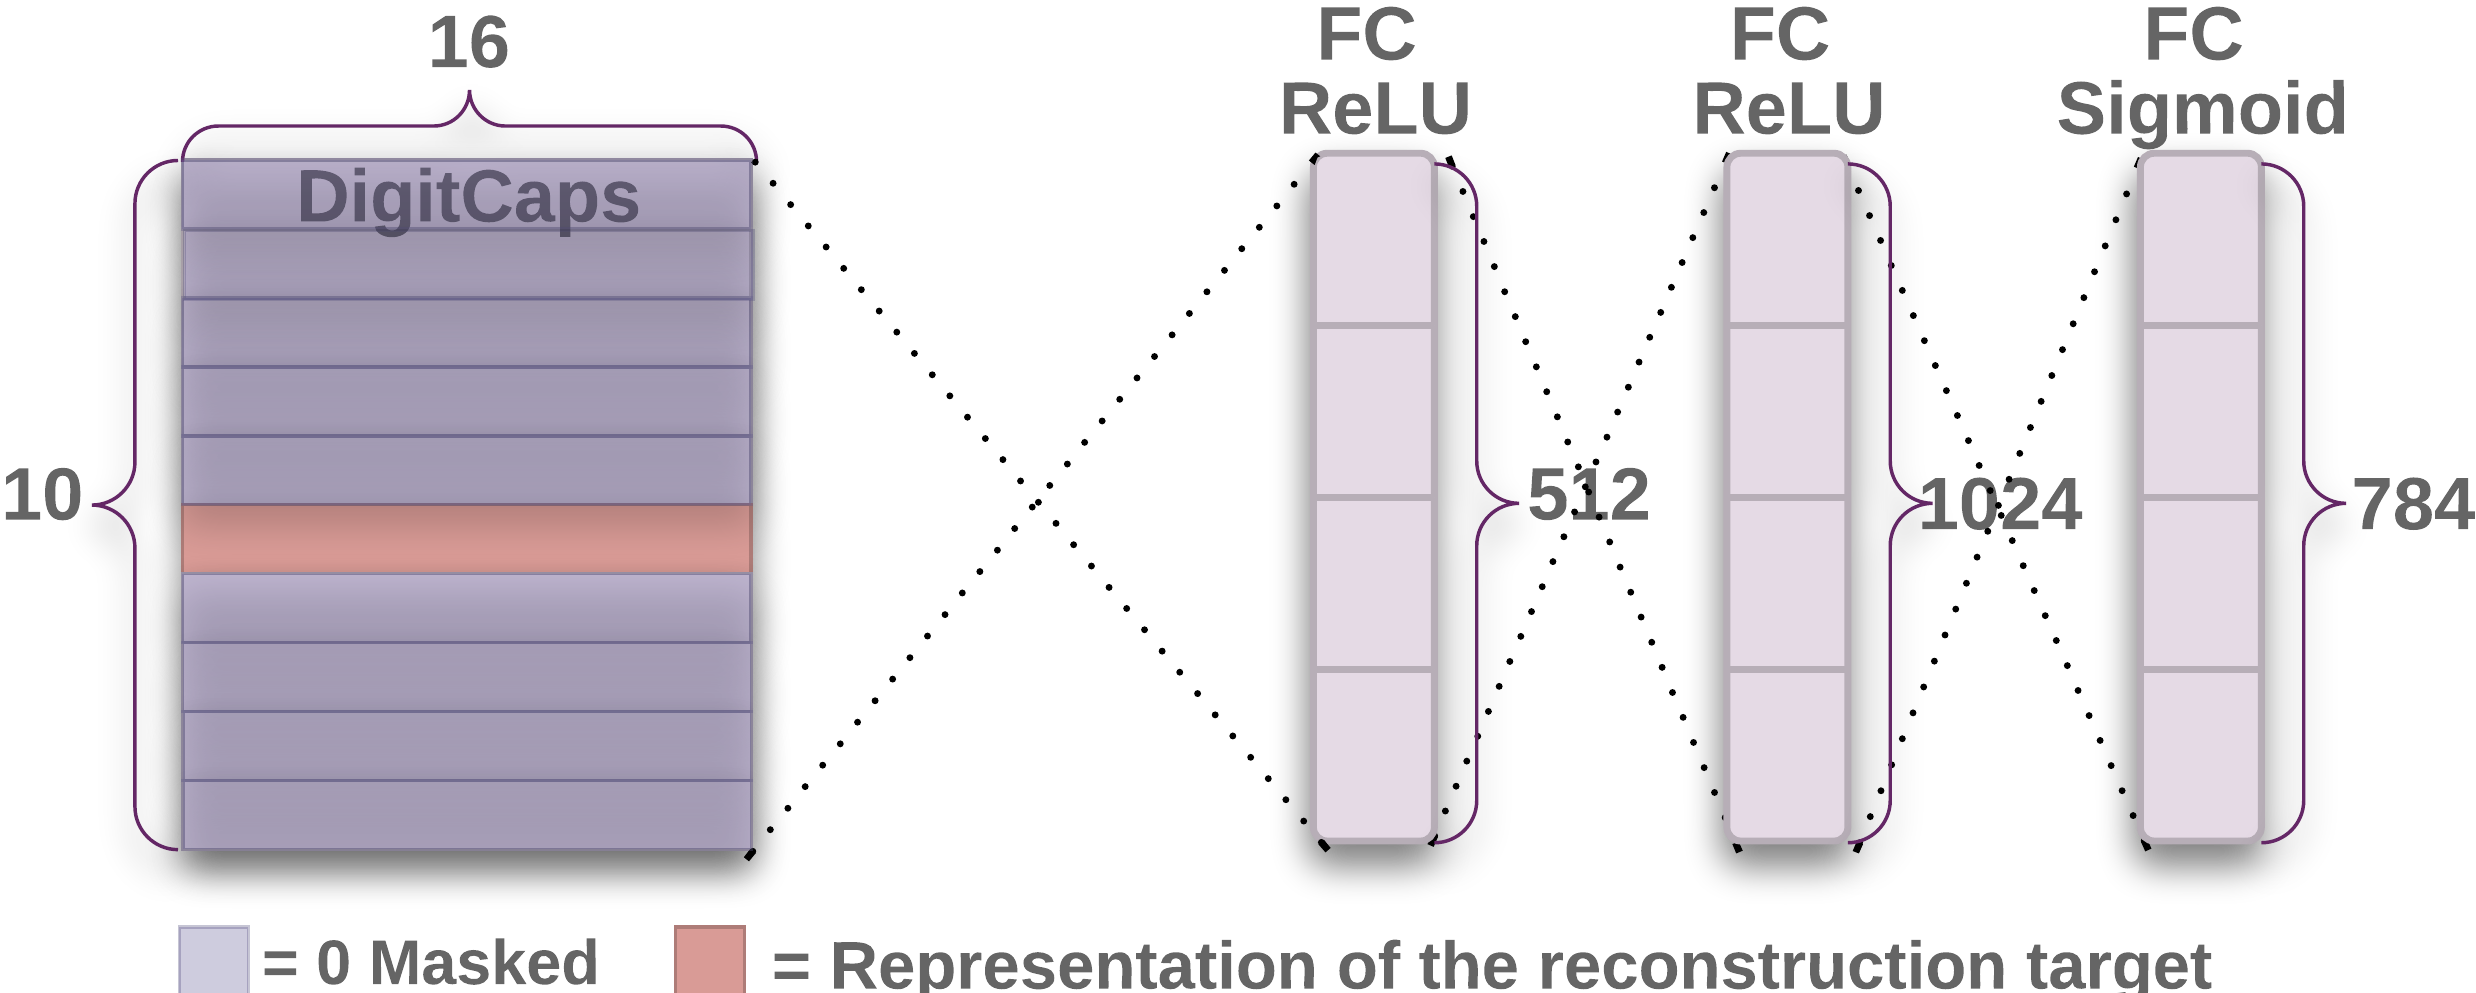
\includegraphics[width=.8\textwidth]{../img/reconsArch.png}
      \end{center}
      \pause

      \begin{itemize}[<+- | alert@+>]
        \item Layer 4: from $16 \times 10$ input to $512$ output, ReLU activations
        \item Layer 5: from $512$ input to $1024$ output, ReLU activations
        \item Layer 6: from $1024$ input to $784$ output, sigmoid activations \\
          {\tiny (after reshaping it produces a $(28 \times 28)$-pixels decoded image)}
      \end{itemize}
    \end{frame}
  }

  \subsection{Architecture: Summary}
  {
    \setbeamertemplate{frame footer}{\colorcite\url{https://d1jnx9ba8s6j9r.cloudfront.net/blog/wp-content/uploads/2017/12/Capsule-Neural-Network-Architecture-Capsule-Networks-Edureka.png}}

    \begin{frame}{Architecture: Summary}
      \begin{center}
        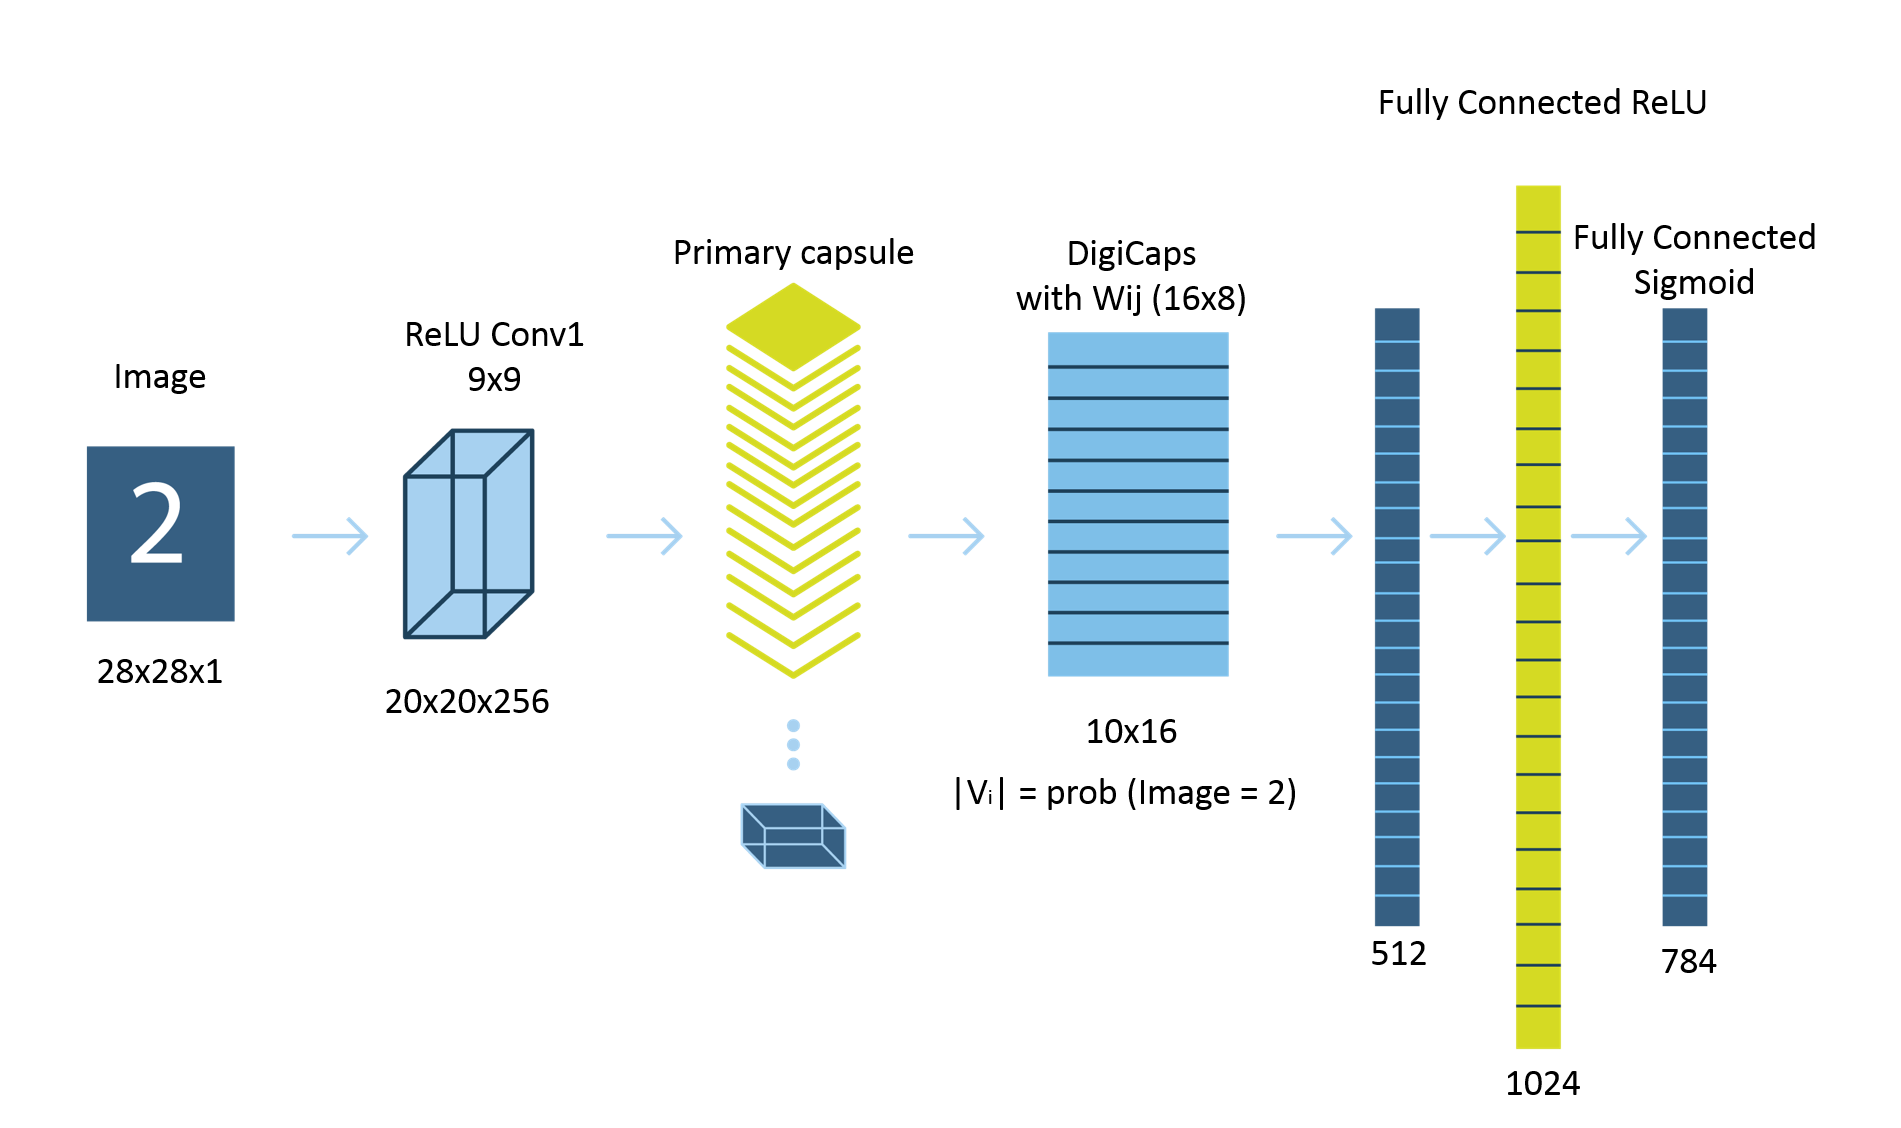
\includegraphics[width=\linewidth]{../img/Capsule-Neural-Network-Architecture-Capsule-Networks-Edureka.png}
      \end{center}
    \end{frame}
  }

%%%%%%%%%%%%%%%%%%%%%%%%%%%%%%%%%%%%%%%%%%%%%%%%%%%%%%%%%%%%%%%%%%%%%%%%%%%%%%%%

  \section{Experiments}

  % TODO show & compare w/ SotA methods
  \subsection{MNIST}
  {
    \setbeamertemplate{frame footer}{\colorcite[\cite{Sabour2017dynamic}]}

    \begin{frame}{MNIST Reconstructions (CapsNet, 3 routing iterations)}
      \begin{tabular}
        { r | c c | c c}
        Label:          & 8 & 5 & 5 & 5 \\
        Prediction:     & 8 & 5 & 3 & 3 \\
        Reconstruction: & 8 & 5 & 5 & 3 \\
        \pbox{.2\textwidth}{\hspace{1em}Input: \\ \\ \\ Output:} &
        \pbox{.2\textwidth}{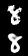
\includegraphics[width=.15\textwidth]{../img/recons/8_226}} &
        \pbox{.2\textwidth}{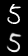
\includegraphics[width=.15\textwidth]{../img/recons/5_153}} &
        \pbox{.2\textwidth}{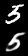
\includegraphics[width=.15\textwidth]{../img/recons/5_2035}} &
        \pbox{.2\textwidth}{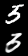
\includegraphics[width=.15\textwidth]{../img/recons/5_2035p}}
      \end{tabular}
    \end{frame}

    \begin{frame}{Dimension Perturbations}
      one of the $16$ dimensions, by intervals of $0.05$ in the range $[-0.25, 0.25]$:
      \pause

      \begin{tabular}{r | r}
        Interpretation & Reconstructions after perturbing \\
        \hline
        ``scale and thickness'' & 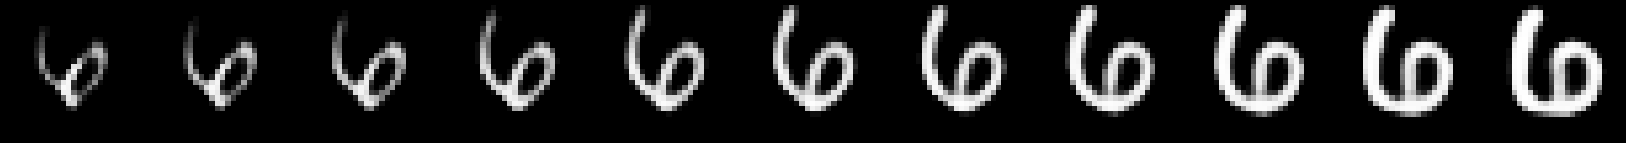
\includegraphics[width=7cm]{../img/recons/dim6} \\
        ``localized part'' & 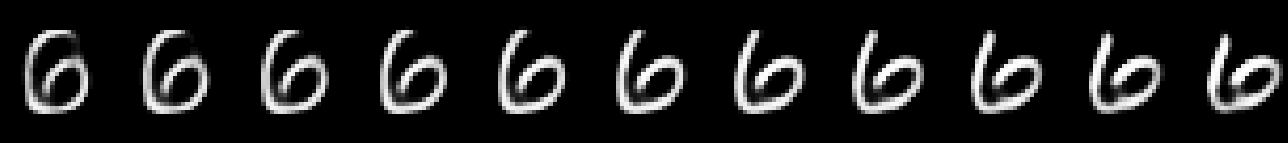
\includegraphics[width=7cm]{../img/recons/dim7} \\
        \pause
        ``stroke thickness'' & 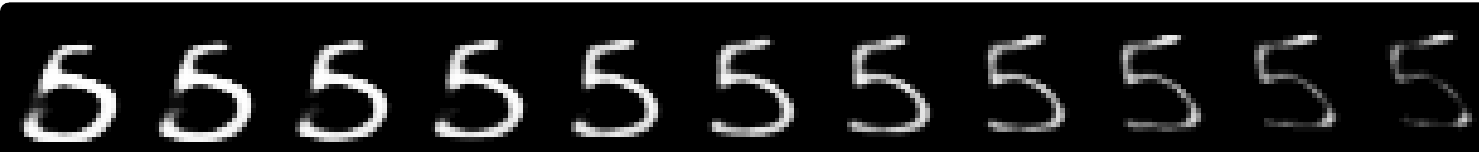
\includegraphics[width=7cm]{../img/recons/dim8} \\
        ``localized skew'' & 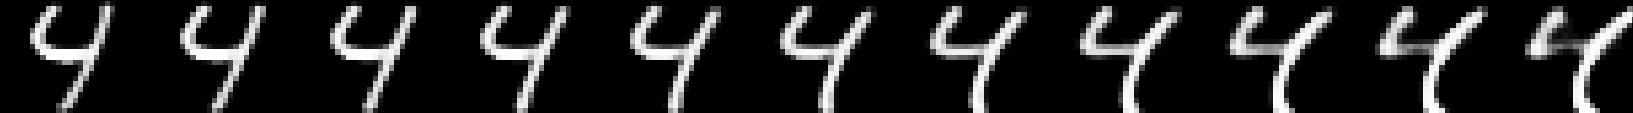
\includegraphics[width=7cm]{../img/recons/dim12} \\
        \pause
        ``width and translation'' & 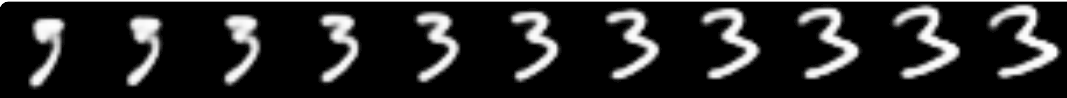
\includegraphics[width=7cm]{../img/recons/dim10} \\
        ``localized part'' & 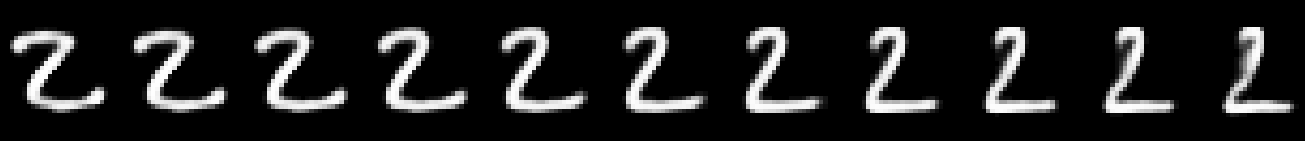
\includegraphics[width=7cm]{../img/recons/dim11}
      \end{tabular}
    \end{frame}
  }

  {
    \setbeamertemplate{frame footer}{\colorcite\url{https://github.com/XifengGuo/CapsNet-Keras}}

    \begin{frame}{Dimension Perturbations: Latent Codes of $0$ and $1$}
      \tiny
      rows: DigitCaps dimensions

      columns (from left to right): $+ \  \{ -0.25, -0.2, -0.15, -0.1, -0.05, 0, 0.05, 0.1, 0.15, 0.2, 0.25 \}$

      \begin{center}
        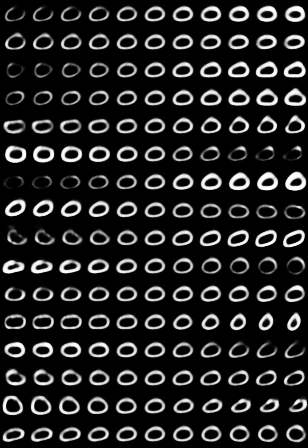
\includegraphics[width=.4\textwidth]{../img/recons-capsnet-keras/manipulate-0.png}
        \includegraphics[width=.4\textwidth]{../img/recons-capsnet-keras/manipulate-1.png}
      \end{center}
    \end{frame}

    \begin{frame}{Dimension Perturbations: Latent Codes of $2$ and $3$}
      \tiny
      rows: DigitCaps dimensions

      columns (from left to right): $+ \  \{ -0.25, -0.2, -0.15, -0.1, -0.05, 0, 0.05, 0.1, 0.15, 0.2, 0.25 \}$

      \begin{center}
        \includegraphics[width=.4\textwidth]{../img/recons-capsnet-keras/manipulate-2.png}
        \includegraphics[width=.4\textwidth]{../img/recons-capsnet-keras/manipulate-3.png}
      \end{center}
    \end{frame}

    \begin{frame}{Dimension Perturbations: Latent Codes of $4$ and $5$}
      \tiny
      rows: DigitCaps dimensions

      columns (from left to right): $+ \  \{ -0.25, -0.2, -0.15, -0.1, -0.05, 0, 0.05, 0.1, 0.15, 0.2, 0.25 \}$

      \begin{center}
        \includegraphics[width=.4\textwidth]{../img/recons-capsnet-keras/manipulate-4.png}
        \includegraphics[width=.4\textwidth]{../img/recons-capsnet-keras/manipulate-5.png}
      \end{center}
    \end{frame}

    \begin{frame}{Dimension Perturbations: Latent Codes of $6$ and $7$}
      \tiny
      rows: DigitCaps dimensions

      columns (from left to right): $+ \  \{ -0.25, -0.2, -0.15, -0.1, -0.05, 0, 0.05, 0.1, 0.15, 0.2, 0.25 \}$

      \begin{center}
        \includegraphics[width=.4\textwidth]{../img/recons-capsnet-keras/manipulate-6.png}
        \includegraphics[width=.4\textwidth]{../img/recons-capsnet-keras/manipulate-7.png}
      \end{center}
    \end{frame}

    \begin{frame}{Dimension Perturbations: Latent Codes of $8$ and $9$}
      \tiny
      rows: DigitCaps dimensions

      columns (from left to right): $+ \  \{ -0.25, -0.2, -0.15, -0.1, -0.05, 0, 0.05, 0.1, 0.15, 0.2, 0.25 \}$

      \begin{center}
        \includegraphics[width=.4\textwidth]{../img/recons-capsnet-keras/manipulate-8.png}
        \includegraphics[width=.4\textwidth]{../img/recons-capsnet-keras/manipulate-9.png}
      \end{center}
    \end{frame}
  }

  \subsection{MultiMNIST}
  {
    \setbeamertemplate{frame footer}{\colorcite[\cite{Sabour2017dynamic}]}

    \begin{frame}{MultiMNIST Reconstructions (CapsNet, 3 routing iterations)}
      \begin{center}
        \begin{tabular}{c c c c}
          R:$(2,7)$ & R:$(6,0)$ & R:$(6,8)$ & R:$(7,1)$ \\
          L:$(2,7)$ & L:$(6,0)$ & L:$(6,8)$ & L:$(7,1)$ \\
          \includegraphics[height=.3\textheight]{../img/recons/27} &
          \includegraphics[height=.3\textheight]{../img/recons/60} &
          \includegraphics[height=.3\textheight]{../img/recons/68} &
          \includegraphics[height=.3\textheight]{../img/recons/71} \\
          \pause
          *R:$(5,7)$ & *R:$(2,3)$ & R:$(2,8)$ & R:P:$(2,7)$ \\
           L:$(5,0)$ &  L:$(4,3)$ & L:$(2,8)$ & L:$(2,8)$ \\
          \includegraphics[height=.3\textheight]{../img/recons/0_5_5_0_332} &
          \includegraphics[height=.3\textheight]{../img/recons/4_3_3_4_397} &
          \includegraphics[height=.3\textheight]{../img/recons/2_8_2_7_152} &
          \includegraphics[height=.3\textheight]{../img/recons/2_8_2_7_153p}
        \end{tabular}
      \end{center}
    \end{frame}

    \begin{frame}{MultiMNIST Reconstructions (CapsNet, 3 routing iterations)}
      \begin{center}
        \begin{tabular}{c c c c}
          R:$(8,7)$ & R:$(9,4)$ & R:$(9,5)$ & R:$(8,4)$ \\
          L:$(8,7)$ & L:$(9,4)$ & L:$(9,5)$ & L:$(8,4)$ \\
          \includegraphics[height=.3\textheight]{../img/recons/87} &
          \includegraphics[height=.3\textheight]{../img/recons/94} &
          \includegraphics[height=.3\textheight]{../img/recons/95} &
          \includegraphics[height=.3\textheight]{../img/recons/84} \\
          \pause
          *R:$(0,8)$ & *R:$(1,6)$ & R:$(4,9)$ &  R:P:$(4, 0)$ \\
           L:$(1,8)$ &  L:$(7,6)$ & L:$(4, 9)$ & L:$(4, 9)$ \\
          \includegraphics[height=.3\textheight]{../img/recons/1_8_8_1_264} &
          \includegraphics[height=.3\textheight]{../img/recons/7_6_6_7_4} &
          \includegraphics[height=.3\textheight]{../img/recons/4_9_4_0_453} &
          \includegraphics[height=.3\textheight]{../img/recons/4_9_4_0_454p}
        \end{tabular}
      \end{center}
    \end{frame}
  }

  \subsection{CIFAR10}

  \subsection{smallNORB}

  \subsection{SVHN}

%%%%%%%%%%%%%%%%%%%%%%%%%%%%%%%%%%%%%%%%%%%%%%%%%%%%%%%%%%%%%%%%%%%%%%%%%%%%%%%%

  \section{Conclusion}

  \subsection{Explanation of Capsules' Efficiency}

  \begin{frame}[standout]
    \begin{center}
      Thank you!

      Questions?
    \end{center}
  \end{frame}

%%%%%%%%%%%%%%%%%%%%%%%%%%%%%%%%%%%%%%%%%%%%%%%%%%%%%%%%%%%%%%%%%%%%%%%%%%%%%%%%

  \appendix
  \begin{frame}[standout]
    Backup Slides
  \end{frame}

  % TODO display (I), (II) instead of i, ii
  \begin{frame}[allowframebreaks]{Further Reading}
    \tiny
    % TODO fill in relevant Further Reading
    % Machine Learning:
    % \begin{itemize}
    %   \item \textbf{Deep Learning} (\cite{Lecun2015deep})
    %   \item \textbf{Deep Learning course} \url{https://www.udacity.com/course/deep-learning--ud730}
    % \end{itemize}
  \end{frame}

  \begin{frame}[allowframebreaks]{References}
    \tiny
    \printbibliography[heading=none]
  \end{frame}

\end{document}
